\documentclass{uai2023} 

\usepackage[american]{babel}


\usepackage{natbib} \bibliographystyle{plainnat}
    \renewcommand{\bibsection}{\subsubsection*{References}}
\usepackage{booktabs} 

\relax \newif\ifmarginprooflinks 
    	\marginprooflinkstrue


\newif\ifbiblatex
        \biblatexfalse

\relax \ifbiblatex
	\usepackage[backend=biber, style=authoryear]{biblatex}
	\DeclareLanguageMapping{american}{american-apa}


	\DeclareFieldFormat{citehyperref}{\DeclareFieldAlias{bibhyperref}{noformat}\bibhyperref{#1}}

	\DeclareFieldFormat{textcitehyperref}{\DeclareFieldAlias{bibhyperref}{noformat}\bibhyperref{#1\ifbool{cbx:parens}
	      {\bibcloseparen\global\boolfalse{cbx:parens}}
	      {}}}

	\savebibmacro{cite}
	\savebibmacro{textcite}

	\renewbibmacro*{cite}{\printtext[citehyperref]{\restorebibmacro{cite}\usebibmacro{cite}}}

	\renewbibmacro*{textcite}{\ifboolexpr{
	    ( not test {\iffieldundef{prenote}} and
	      test {\ifnumequal{\value{citecount}}{1}} )
	    or
	    ( not test {\iffieldundef{postnote}} and
	      test {\ifnumequal{\value{citecount}}{\value{citetotal}}} )
	  }
	    {\DeclareFieldAlias{textcitehyperref}{noformat}}
	    {}\printtext[textcitehyperref]{\restorebibmacro{textcite}\usebibmacro{textcite}}}

	\DeclareCiteCommand{\brakcite}
	  {\usebibmacro{prenote}}
	  {\usebibmacro{citeindex}\printtext[bibhyperref]{[\usebibmacro{cite}]}}
	  {\multicitedelim}
	  {\usebibmacro{postnote}}
    \else
    \let\parencite\citep
    \let\textcite\citet
    \fi

\relax \usepackage[dvipsnames]{xcolor}
\usepackage{mathtools}
    \usepackage{amssymb}
		\DeclareMathSymbol{\shortminus}{\mathbin}{AMSa}{"39}
\usepackage{bbm}
\usepackage{faktor}
\usepackage{graphicx}
    \usepackage{scalerel}
    \usepackage{enumitem}
    \usepackage{nicefrac}\let\nf\nicefrac

\usepackage{hyperref} \hypersetup{colorlinks=true, linkcolor=blue!75!black, urlcolor=magenta, citecolor=green!50!black}

\usepackage{tikz}
	\usetikzlibrary{positioning,fit,calc, decorations, arrows, shapes, shapes.geometric}
	\usetikzlibrary{cd}

\tikzset{AmpRep/.style={ampersand replacement=\&}}
	\tikzset{center base/.style={baseline={([yshift=-.8ex]current bounding box.center)}}}
	\tikzset{paperfig/.style={center base,scale=0.9, every node/.style={transform shape}}}

\tikzset{dpadded/.style={rounded corners=2, inner sep=0.7em, draw, outer sep=0.3em, fill={black!50}, fill opacity=0.08, text opacity=1}}
	\tikzset{dpad0/.style={outer sep=0.05em, inner sep=0.3em, draw=gray!75, rounded corners=4, fill=black!08, fill opacity=1, align=center}}
	\tikzset{dpadinline/.style={outer sep=0.05em, inner sep=2.5pt, rounded corners=2.5pt, draw=gray!75, fill=black!08, fill opacity=1, align=center, font=\small}}

 	\tikzset{dpad/.style args={#1}{every matrix/.append style={nodes={dpadded, #1}}}}
	\tikzset{light pad/.style={outer sep=0.2em, inner sep=0.5em, draw=gray!50}}

	\tikzset{arr/.style={draw, ->, thick, shorten <=3pt, shorten >=3pt}}
	\tikzset{arr0/.style={draw, ->, thick, shorten <=0pt, shorten >=0pt}}
	\tikzset{arr1/.style={draw, ->, thick, shorten <=1pt, shorten >=1pt}}
	\tikzset{arr2/.style={draw, ->, thick, shorten <=2pt, shorten >=2pt}}

	\newcommand\cmergearr[5][]{
		\draw[arr, #1, -] (#2) -- (#5) -- (#3);
		\draw[arr, #1, shorten <=0] (#5) -- (#4);
		}
	\newcommand\mergearr[4][]{
		\coordinate (center-#2#3#4) at (barycentric cs:#2=1,#3=1,#4=1.2);
		\cmergearr[#1]{#2}{#3}{#4}{center-#2#3#4}
		}
	\newcommand\cunmergearr[5][]{
		\draw[arr, #1, -, shorten >=0] (#2) -- (#5);
		\draw[arr, #1, shorten <=0] (#5) -- (#3);
		\draw[arr, #1, shorten <=0] (#5) -- (#4);
		}
	\newcommand\unmergearr[4][]{
		\coordinate (center-#2#3#4) at (barycentric cs:#2=1.2,#3=1,#4=1);
		\cunmergearr[#1]{#2}{#3}{#4}{center-#2#3#4}
		}

\usepackage{amsthm,thmtools} \usepackage[noabbrev,nameinlink,capitalize]{cleveref}
    \theoremstyle{plain}
    \newtheorem{theorem}{Theorem}
	\newtheorem{coro}{Corollary}[theorem]
    \newtheorem{prop}[theorem]{Proposition}
    \newtheorem{conj}[theorem]{Conjecture}
    \newtheorem{claim}{Claim}
    \newtheorem{remark}{Remark}
    \newtheorem{lemma}[theorem]{Lemma}
    \theoremstyle{definition}
\declaretheorem[name=Definition, qed=$\square$]{defn}
\declaretheorem[name=Example, qed=$\square$]{example}

    \definecolor{openQcolor}{rgb}{0.9,0.2,0.9}
    \declaretheorem[preheadhook=\color{openQcolor},name=Open Question]{openQ}

	\crefname{defn}{Definition}{Definitions}
	\crefname{prop}{Proposition}{Propositions}
    \crefname{issue}{Issue}{Issues}

\relax \let\Horig\H
	\let\H\relax
	\DeclareMathOperator{\H}{\mathrm{H}} \DeclareMathOperator{\I}{\mathrm{I}} \DeclareMathOperator*{\Ex}{\mathbb{E}} \DeclareMathOperator*{\EX}{\scalebox{1.5}{$\mathbb{E}$}}
    \newcommand{\ifrac}[2]{{#1}/{#2}}

\DeclareMathOperator*{\argmin}{\arg\!\min}
    \DeclareMathOperator*{\argmax}{\arg\!\max}

    \newcommand{\mat}[1]{\mathbf{#1}}
    \DeclarePairedDelimiterX{\infdivx}[2]{(}{)}{#1\;\delimsize\|\;#2}
	\newcommand{\thickD}{I\mkern-8muD}
	\newcommand{\kldiv}{\thickD\infdivx}
	\newcommand{\tto}{\rightarrow\mathrel{\mspace{-15mu}}\rightarrow}

	\newcommand{\datadist}[1]{\Pr\nolimits_{#1}}


	\makeatletter
	\newcommand{\subalign}[1]{\vcenter{\Let@ \restore@math@cr \default@tag
	    \baselineskip\fontdimen10 \scriptfont\tw@
	    \advance\baselineskip\fontdimen12 \scriptfont\tw@
	    \lineskip\thr@@\fontdimen8 \scriptfont\thr@@
	    \lineskiplimit\lineskip
	    \ialign{\hfil$\m@th\scriptstyle##$&$\m@th\scriptstyle{}##$\hfil\crcr
	      #1\crcr
	    }}}
	\makeatother
	\newcommand\numberthis{\addtocounter{equation}{1}\tag{\theequation}}

\relax \newcommand{\ssub}[1]{_{\!_{#1}\!}}
\newcommand{\bp}[1][L]{\mat{p}\ssub{#1}}
	\newcommand{\bP}[1][L]{\mat{P}\ssub{#1}}
	\newcommand{\V}{\mathcal V}
	\newcommand{\N}{\mathcal N}
	\newcommand{\Ed}{\mathcal E}

    \newcommand{\balpha}{\boldsymbol\alpha}
    \newcommand{\bbeta}{\boldsymbol\beta}

	\DeclareMathAlphabet{\mathdcal}{U}{dutchcal}{m}{n}
	\DeclareMathAlphabet{\mathbdcal}{U}{dutchcal}{b}{n}
	\newcommand{\dg}[1]{\mathbdcal{#1}}
	\newcommand{\PDGof}[1]{{\dg M}_{#1}}
	\newcommand{\UPDGof}[1]{{\dg N}_{#1}}
	\newcommand\VFE{\mathit{V\mkern-4mu F\mkern-4.5mu E}}

	\newcommand\Inc{\mathit{Inc}}
	\newcommand{\IDef}[1]{\mathit{IDef}_{\!#1}}
\newcommand{\ed}[3]{#2\overset{\smash{\mskip-5mu\raisebox{-1pt}{$\scriptscriptstyle
	        #1$}}}{\rightarrow} #3}

    \newcommand{\nhphantom}[2]{\sbox0{\kern-2\nulldelimiterspace$\left.\delimsize#1\vphantom{#2}\right.$}\hspace{-.97\wd0}}
\makeatletter
	\newsavebox{\abcmycontentbox}
	\newcommand\DeclareDoubleDelim[5]{
	    \DeclarePairedDelimiterXPP{#1}[1]{\sbox{\abcmycontentbox}{\ensuremath{##1}}}{#2}{#5}{}{\nhphantom{#3}{\usebox\abcmycontentbox}\hspace{1.2pt} \delimsize#3\mathopen{}\usebox{\abcmycontentbox}\mathclose{}\delimsize#4\hspace{1.2pt}\nhphantom{#4}{\usebox\abcmycontentbox}}}
	\makeatother
	\DeclareDoubleDelim
		\SD\{\{\}\}
	\DeclareDoubleDelim
		\bbr[[]]
\makeatletter
	\newsavebox{\aar@content}
	\newcommand\aar{\@ifstar\aar@one@star\aar@plain}
	\newcommand\aar@one@star{\@ifstar\aar@resize{\aar@plain*}}
	\newcommand\aar@resize[1]{\sbox{\aar@content}{#1}\scaleleftright[3.8ex]
		{\Biggl\langle\!\!\!\!\Biggl\langle}{\usebox{\aar@content}}
		{\Biggr\rangle\!\!\!\!\Biggr\rangle}}
	\DeclareDoubleDelim
		\aar@plain\langle\langle\rangle\rangle
	\makeatother
    
\relax \newcommand\Bel{\mathrm{Bel}}
    \newcommand\Plaus{\mathrm{Plaus}}




\relax \usepackage{xpatch}
	\makeatletter
	\xpatchcmd{\thmt@restatable}{\csname #2\@xa\endcsname\ifx\@nx#1\@nx\else[{#1}]\fi}{\ifthmt@thisistheone\csname #2\@xa\endcsname\ifx\@nx#1\@nx\else[{#1}]\fi
	   \else\fi}
	   {}{\typeout{FIRST PATCH TO THM RESTATE FAILED}} \xpatchcmd{\thmt@restatable}{\csname end#2\endcsname}
	   {\ifthmt@thisistheone\csname end#2\endcsname\else\fi}
	   {}{\typeout{FAILED SECOND THMT RESTATE PATCH}}

\newcommand{\recall}[1]{\medskip\par\noindent{\bf \Cref{thmt@@#1}.} \begingroup\em \noindent
	   \expandafter\csname#1\endcsname* \endgroup\par\smallskip}

   	\setlength\marginparwidth{1.55cm}
	\newenvironment{linked}[3][]{\def\linkedproof{#3}\def\linkedtype{#2}\ifmarginprooflinks
		\marginpar{\vspace{1.5em}
			\centering \hyperref[proof:\linkedproof]{\color{blue!30!white}\scaleleftright{$\Big[$}{\,\mbox{\footnotesize\centering\tt\begin{tabular}{@{}c@{}}
link to\\[-0.15em]
				proof
			\end{tabular}}\,}{$\Big]$}}~
			}\fi
        \restatable[#1]{#2}{#2:#3}\label{#2:#3}}{\endrestatable }
	\makeatother
		\newcounter{proofcntr}
		\newenvironment{lproof}{\begin{proof}\refstepcounter{proofcntr}}{\end{proof}}

		\usepackage{cancel}
		\newcommand{\Cancel}[2][black]{{\color{#1}\cancel{\color{black}#2}}}

		\usepackage{tcolorbox}
		\tcbuselibrary{most}
		\tcolorboxenvironment{lproof}{
enhanced,
			parbox=false,
			boxrule=0pt,
			frame hidden,
			borderline west={4pt}{0pt}{blue!20!black!40!white},
colback={blue!20!black!05!white},
			sharp corners,
			breakable,
}
\newcommand{\begthm}[3][]{\begin{#2}[{name=#1},restate=#3,label=#3]}

\relax \newcommand{\TODO}[1][INCOMPLETE]{{\centering\Large\color{red}$\langle$~\texttt{#1}~$\rangle$\par}}
    \newcommand{\dfootnote}[1]{\let\oldthefootnote=\thefootnote \setcounter{footnote}{999}
        \renewcommand{\thefootnote}{\textdagger}\footnote{#1}\let\thefootnote=\oldthefootnote }
	\newcommand{\dfootnotemark}{
		\footnotemark[999]
	}


\definecolor{brownish}{rgb}{0.5, 0.2, 0.1}
\newtcolorbox{wip}{colback=brownish!20!white,title={$\langle$under construction$\rangle$},enhanced jigsaw,
    breakable,
colframe=brownish!40!white,}
\newtcolorbox{phaseout}{colback={gray!02!white},
    coltext={gray!35!white},
    colframe={red!02!white},
    coltitle={red!35!white},
title={~\hfill(depricated)},
    enhanced jigsaw,
fontupper=\small,
    parbox=false,
    boxrule=0pt,
sharp corners,
    breakable
}

\newtcolorbox{computation}{colback={white},
enhanced jigsaw,
fontupper=\Large\itshape,
    fontlower=\small,
    parbox=false,
    boxrule=0pt,
    frame hidden,
    borderline west={4pt}{0pt}{green!20!black!40!white},
    sharp corners,
    breakable,
enlarge left by=-4em,
    enlarge right by=4em,
    width=\linewidth+8em
}

\newtcbtheorem[use counter=example]{examplex}{Example}{
        label type=example,
        fonttitle=\bfseries,
enhanced jigsaw,
before=\par\medskip\noindent,
parbox=false,
colback=white,
        sharp corners,
        breakable,
}
{ex}


\makeatletter
\newcommand{\@minipagerestore}{\setlength{\parskip}{\medskipamount}}
\makeatother

\usepackage{xparse}
\let\realItem\item \makeatletter
\NewDocumentCommand\myItemboldperiod{o}{\IfNoValueTF{#1}{\realItem}{\realItem[\textbf{#1.}]\def\@currentlabel{#1}\protected@edef\cref@currentlabel{[CFaxiomsi][][]#1}}}
\makeatother


\newlist{CFaxioms}{enumerate}{1}
\setlist[CFaxioms]{
    resume,label=\textbf{CF\arabic{*}.},
ref={CF\arabic*},
leftmargin=2.5em,
    before=\let\item\myItemboldperiod,
    topsep=1ex
    }
\crefname{CFaxiomsi}{}{}
\newcommand\commentout[1]{}
 



\newcommand{\ext}[1]{\overline #1} \newcommand{\Unif}{\mathrm{Unif}}

\newcommand\cofunc{commitment function}
\newcommand\confdom{\mathdcal C}
\newcommand\ZO{\mathrm{ZO}}
\newcommand\Rplus{\mathbb R_+}
\newcommand\X{\mathcal X}



\title{Updating with Confidence
}



\author[1]{\href{mailto:<oer5@cornell.edu>?Subject=confidence-paper}{Oliver E Richardson}{}}
\author[1]{Joseph Y Halpern}
\affil[1]{Computer Science Dept.\\
    Cornell University\\
    Ithaca, New York, USA
}

\begin{document}
\maketitle

\begin{abstract}
We introduce a new notion of confidence, which arises when learning or updating beliefs.
\end{abstract}

\section{Introduction}\label{sec:intro}
\def\stmt{$A$}



\commentout{The ability to articulate a \emph{degree of confidence} 
is a critical aspect of representing knowledge.
	There are 
many well-established ways to quantify (un)certinaty \parencite[\S2]{halpern2017reasoning},
		and chief among them is probability.
	While ``confidence'' can be coherently read in probabilistic terms,
		such usage may shadow another important concept.
	This paper details a different conception that arises when updating beliefs. 
	As we shall see, this notion of confidence
	complements traditional representations of uncertainty (such as probability), 
	and moreover unifies several different concepts across AI.
}

What should it mean to say that one has a high degree of confidence in a statement $\phi$?  It is often taken to mean that we think $\phi$ is likely. 
Here we argue that there is a related but more useful conception of confidence that arises when updating---one that complements likelihood and, moreover, unifies several different concepts in the literature.


For us, confidence is a measure of \emph{trust}, rather than likelihood.
In particular, the {degree of confidence} that one has in a piece of information $\phi$
quantifies how seriously to take $\phi$ in updating one's beliefs. 
So at one extreme,
if we observe $\phi$ but have no confidence in it, 
we should not change our beliefs at all;
at the other, if we have full confidence in $\phi$,
 we should fully incorporate it into our beliefs.
 
\begin{example} \label{ex:prob-simple}
Suppose
our belief state is a probability measure, and $\phi$ is an event. 
A full-confidence update then amounts to conditioning on $\phi$, after which $\phi$ has probability 1, and so cannot be further incorporated.
We also have an obvious way to describe intermediate degrees of confidence:
if we learn $\phi$ with confidence
$\alpha \in [0,1]$
and start with prior probability $\Pr$, then we end up with the
posterior $(1-\alpha)\Pr + \alpha (\Pr\mid \phi)$.
Thus, having high confidence in $\phi$ leads to posterior beliefs that give $\phi$
high
probability.
The converse is false, however, so
confidence and probability can be quite different.
%joe1
%If an untrusted source tells us $\phi$ which we already happen to
If an untrusted source tells us $\phi$, which we already happen to
believe,  
then our prior assigns $\phi$ high probability,
we learn $\phi$ with low confidence,
and our posterior beliefs still give $\phi$ high probability.  
%joe1: I don't know what "more independent" means
%Confidence and prior probability are even more independent:
And
if we learn a surprising fact $\phi$ from a trusted source, we have
high confidence in $\phi$ despite it having low prior probability. 
\end{example}

\commentout{
	In this context, 
	the confidence $\chi \in [0,1]$ has a clear interpretation as the ``fraction of the way towards full incorporation'',
	but in others,
	it may be 
	less clear what a number on this scale (say, $\chi{=}0.7$) means.
}

This notion of confidence applies far more broadly.
We now give an example with the same critical elements,
but a very different flavor.


\begin{example}\label{ex:classifier}
Consider a neural network, whose ``belief state'' is a setting of weights.
For definiteness, suppose we are talking about a classifier, so that for every setting of weights $\theta$, there is a function
$f_\theta : X \to \Delta Y$ that maps inputs $x \in X$ to
%joe1
%distributions $f_\theta(x)$ over possible class lables $Y$.
distributions $f_\theta(x)$ over possible class labels $Y$.  
Modern learning algorithms (like gradient descent) make small incremental changes to the weights.
Therefore, if we update $\theta$ with a labeled training example $\phi = (x,y)$ to obtain new weights $\theta'$, there is no guarantee that $f_{\theta'}(x)$ gives high probability to $y$---only that it will be higher than it was before.
In other words, such algorithms 
(in contrast to their historical counterparts like conjunction learning algorithms \parencite{conjunctions}) 
do not take any one encounter with a training example too seriously---
%joe1
%\unskip that is, they make low-confidence updates.  
\unskip that is, they make low-confidence updates to the belief state
(i.e., the weights).    
This relative distrust of each individual sample is arguably what makes the training process robust to noisy or contradictory observations.
\commentout{
	As a result,
	there is a significant difference between going through the training data once
\unskip, and doing so many times.}


Nevertheless, 
if we train by repeatedly updating with the sample $\phi$, 
the weights do eventually converge.
%joe1: I don't mind white lies in the introduction, as long as experts
%won't be uncomfortable with it
%\footnote{Note for Joe: this is a
%white lie; the truth depends a bit on the architecture, and we may
%require that the space is compact. But this can be easily achieved by
%considering weights taking extended real values.} 
%joe1: We have to explain what "Doing so" means
%Doing so would be an extreme action, and only appropriate if we have
%complete trust in $\phi$, meaning we think important that $x$ always
Updating the weights with weights that have converged and classify $x$
as $y$ would be appropriate only if we have
complete trust in $\phi$, meaning we think important it that $x$ always
be classified as $y$. 
At the opposite extreme, if we have no trust in $\phi$, we should
%joe1
%simply discard it without changing our weights.
simply discard the sample without changing our weights.  
%joe1
%Furthermore, our definition of a full-confidence update 
%already suggests what to do for intermediate levels of confidence:
Our definition of a full-confidence update 
also suggests what to do for intermediate levels of confidence:
simply stop the training process before convergence. 
%joe1: is it really standard to use the same \phi over and over
%again.  This seems strange to me.
%Consequently, the number of training iterations $n$ 
Consequently, the number $n$ of training iterations with $\phi$
functions as a description of 
intermediate levels of confidence: it interpolates
between no confidence (zero iterations) and full confidence
%joe1
%(infinite iterations).
(infinitely many iterations). 

%joe1*: Although I didn't cut this, I don't think this is the
%right place for this point.  Among other things, you've switched out
%of the blue from %confidence being a number in [0,1] to being a number 
%in [0,\infty]
This way of measuring confidence has a convenient property:
first updating with confidence $n$ (that is, performing $n$ training
iterations), 
	and then afterwards updating with confidence $m$ (so $m$ additional iterations),
	is equivalent to a single update with confidence $m+n$.
	We call a measure of confidence that behaves this way \emph{additive}.
\end{example}

%joe1*: I think that making a big fuss about these two ways here is a
%*terrible* idea, as I've indicated often in our conversations.
%You've taken what should be a very minor point, and elevated it to a
%central point in the story.  
We have now seen two very different ways of describing confidence. 
Are they related? 
Should we prefer one style over the other?
The number $\alpha \in [0,1]$ used in \cref{ex:prob-simple}
appears to have an important advantage: an intermediate value can be clearly interpreted as a ``proportion of incorporation'', while the number of training iterations $n$ used in
\cref{ex:classifier} only really has meaning relative to
other values of $n$ for the same training algorithm.
On the other hand,
the apprach taken in the second example
appears to be more general. 
It is not clear that a proportion $\alpha \in [0,1]$ 
is meaningful in \cref{ex:classifier},
but \cref{ex:prob-simple} can be
readily captured by a number of iterations 
$n$, as follows.
If we fix some ``unit confidence'', say $\iota=0.01$,
then for any $n \in \mathbb N$,
sequentially performing $n$ updates of confidence $\iota$ is 
equivalent to a single one of confidence $\alpha= 1-(0.99)^n$.
%joe1* This is true only if we assume additivity, which I see no
%reason to assume in general.  Again, you're taking a minor technical
%point and giving it way too much prominence
Or, inverting:
to specify confidence $\alpha$, it suffices to 
instead give a number
\begin{equation} \label{eq:loglogiota}
 	n = \log (1 - \alpha ) / \log(1-\iota) 
	\quad\in[0,\infty]
\end{equation}
of confidence-$\iota$ updates to be performed in sequence.
\commentout{
	Thus, in contexts where a proportion of incorporation $\alpha\in[0,1]$ is meaningful,
a number of iterations $n$ is meaningful as well, provided the unit
	$\iota$ is understood.
}


In some contexts, both styles of measuring confidence are used. 
To illustrate, 
we turn to another class of examples of confidence
based on the work of 
\citeauthor{shafer1976mathematical},
whose 
\citeyear{shafer1976mathematical} book
was written largely 
to develop a theory of what we have been calling confidence,
based on (and tailored to) to his preferred representation of
uncertainty. 



\begin{example} \label{ex:shafer}
Let $W$ be a finite set of possible worlds, 
and suppose our belief state is a 
\emph{mass function} $m : 2^W \! \to\! [0,1]$
satisfying $\sum_{U \subseteq W} m(U) \!=\! 1$ 
and $m(\emptyset) \!=\! 0$. 
>From $m$, one can obtain 
%joe1
%a Dempster-Shafer belief function,
%which is a generalization of a finite probability measure over $W$, by
a Dempster-Shafer belief function $\Bel_m$ 
(belief functions are generalization probability measures), by defining
$\Bel_m(U) = \sum_{V \subseteq U} m(V)$
\parencite{shafer1976mathematical}.

%joe1: why introduce new terminology (evidence that supports an event
%\phi) on top of the terminology we already have (confidence).  And
%now you're back to viewing confidence as being in [0,1]!  This switch
%back and forth is really bad for the reader.
%Suppose we come accross evidence that supports an event $\phi
Suppose that learn $\phi 
\subseteq W$ with confidence $\alpha \in [0,1]$.  
%joe1
%Together, $\phi$ and our confidence $\alpha$ in it
Shafer suggests that $\phi$ and our confidence $\alpha$ in it
%joe1: 
%can be represented by another mass function $s$
can be represented by another mass function $s^\phi_\alpha$,
called a \emph{simple support function},
that places $\alpha$ of its mass on $\phi$, and the rest on the trivial event $W$.
%joe1
%To combine our prior belief $m$ with the new evidence $s$,
To combine our prior belief $m$ with the new evidence $s_\phi^\alpha$,
Shafer argues we should use Dempster's rule of combination,
%joe1
%to obtain a posterior $m' := m \oplus s$,
to obtain a posterior mass function $m_\phi^\alpha := m \oplus
s\phi^\alpha$,  
given in this case by:
%joe1*: this is getting far too much into the weeds for an introduction.
%This should be shortned, and said without the technical details.
\begin{align*}
%joe1
  %  m'(U) &=
    m_\phi^\alpha(U) &= 
\frac{1}{\!\displaystyle 1 - \alpha \sum_{\mathclap{V \subseteq (W \setminus \phi)}} m(V)\!}
	\Big(
	(1-\alpha) m(U) + 
	\alpha \sum_{\substack{\mathclap{V \subseteq W} \\ \mathllap{V \cap \phi} = \mathrlap{U}}} m(U) 
		\Big).
\end{align*}
It is easy to verify that
%joe1
%when $\alpha = 0$, the posterior beliefs are the same as the
%prior ones, and that when $\alpha = 1$,
%all mass is assigned to subsets of $\phi$.
$m_\phi^0 = m$ (so when $\alpha = 0$, the posterior beliefs are the
same as the prior beliefs) and $m_\phi^1$ 
assigns all mass to subsets of $\phi$.
%joe1
%It follows that, after the update, $\Bel_{m'}(\phi)$.
It follows that, after the update, $\Bel_{m_\phi^1}(\phi) = 1$.
So again, we have two extremes in confidence, continuously parameterized
by a value $\alpha \in [0,1]$.


We now look at some special cases. Suppose that $\Bel_m$ is a probability 
measure $\Pr$, or equivalently, that $m$ only assigns mass to singletons.
%joe1
%Then $m'$ also only assigns mass to singletons, and is given by:
Then $m_\phi^\alpha$ also assigns mass to only singletons, and is given by:
\begin{equation}
%joe1
  %  m'(\{x\}) =
    m_\phi^\alpha(\{x\}) =
\frac{\alpha\; \Pr(\{x\} \cap \phi) + (1-\alpha)\, \Pr(\{x\})}{1 - \alpha + \alpha\; \Pr(\phi)}.
\end{equation}
%joe1
%As a function of $\alpha \in [0,1]$, $m'$ is
Thus, as a function of $\alpha \in [0,1]$, $m_\phi^\alpha$ is  
a path that begins at $\Pr$,  ends at $(\Pr |\phi)$,
and can even be viewed as a ``proportion of the way to incorporation'',
just like in \cref{ex:prob-simple}.
But it is parameterized differently.
Thus, we need more assumptions in order to pin down the
exact meaning of an intermediate confidence value.
In \cref{sec:loss-repr}, we will
develop tools we need to fully understand the relationship between
these two paths from $\Pr$ to $\Pr|\phi$, and the sense in which
each one is natural.

%joe1*: This paragraph should be greatly shortened (or cut).  It goes
%way too much into the weeds.  I actually don't even understand what you
%wrote, and I have a fair amount of expertise in belief functions 
Alternatively, suppose that $m$ is not a probability but rather
another simple support function on $\phi$. 
Then so is $m' = m\oplus s$. 
How much total evidence for $\phi$ does $m'$ represent?
%joe1: I have no idea where "overwhelmingly standard" is coming from
%Byu definition, the measure of the union of two disjoint sets is the
%sum of the measure of each set, but we have no obvious analogue of
%disjoint set.
%It is overwhelmingly standard to have a measurement that combines
%additively: 
%if you had three (distinct) gallons of water and get another, you now
%have four; 
%if you had six (independent) random bits and get three more, you now
%have nine.  
What would be necessary to get an additive measurement confidence, 
for simple support functions? 
Shafer calls such a quantity \emph{weight of evidence},
and proves that that of $s$ must be of the form
$w = k \log (1-\alpha)$ for some $k < 0$
[\citeauthor[pg 78]{shafer1976mathematical}]. 
Note that this is precisely the expression for $t$
in \eqref{eq:loglogiota}, 
because a choice of $\iota < 1$
is equivalent to a choice of $k = \log(1-\iota) < 0$.
Weight of evidence is
not just additive;
it also plays a fundemental role in the theory of belief
functions.
For example, it provides a
canonical (and minimal) way of decomposing
combined evidence into simple support functions
[\citeauthor[Theorem 5.5]{shafer1976mathematical}].
\end{example}

%joe1: Where have we said that Shafer gives two reprsentations of
%confidence?  Does Shafer view these as two reprsentations of
%confidence?  I doubt it.  Why on earth does this have anything to
%owith low-confidence observations.   You may have some intuitons
%here, but you certainly haven't revealed them to the reader.
Shafer's two different representations of confidence---the
degree of support $\alpha$ and the weight of evidence $w$---address
a real difficulty with the Bayesian formalism: how to handle
low-confidence observations gracefully. 
However, this theory only applies in an increasingly esoteric paradigm in which
one's mental state is a Dempster-Shafer belief function. 
The present paper, and the general notion of confidence we
formalize in \cref{sec:updateformalism}, can be thought of a vast
generalization of Shafer's handling of this problem to any setting
where beliefs satisfy some minimal assumptions.

%joe1*: You haven't really discussed the issue of "objecgive meaning"
%at all!  We have certainly not seen any such evidence.
In three places now we have seen evidence suggesting that 
additive descriptions of confidence do not have objective meaning,
but rather are only meaningful relative to some inscrutible choice.
The meaning of $n$ in \cref{ex:classifier} depends on the learning algorithm,
the quantity in \eqref{eq:loglogiota} requires an irrelevant choice of $\iota$,
and the weight of evidence is only unique up to the constant $k$.
However, we will see in \cref{sec:vecrep} that insofar as there is an 
%joe1*: What makes it "natural"?  Why shuld small values of n (which
%means going to the [0,\infty) scale and small values of
%\alpha be indistiguishable.  You have provided no intuition
%whatsoever for why this should be true. 
$\alpha$ with an objective meaning, there is also a natural additive 
scale for confidence: the unique one for which small values of $n$ and 
small values of $\alpha$ are indistinguishable, or equivalently,
the unique base for which derivatives of $\alpha$ and $n$ with respect
to one another (or any third quantity) identical.
%joe1*: I care about confidence. What makes this natural?  This seems
%like an extremely technical mathematical property.
Thus, there is a special scale of additive confidence $n \in [0,\infty]$
for the same reason that there is natural base for exponentiation: 
it is the only base whose differential at 0 is the identity. 
(Indeed in these simple cases, this amounts to taking $k = -\log e$
and $\iota = 1-\frac1e$ so that all logarithms are base $e$---but at a
deeper level, this is a consequence of the uniqueness of the
%joe1*: Lie algebras come completely out of the blue.  This is a paper
%on confidence!  
exponential map of the Lie algebra implicit in our framework.) 
To summarize: there is a unique way to represent a confidence
%joe1*: Again, you're making what I view as a minor technicality a
%central part of the story, and making it the basis for your "natural"
%representaion.  I *strongly* object.
$\alpha \in [0,1]$ as a confidence $\beta \in [0, \infty]$
such that the two scales behave identically when both are small. 
But the intuition behind additive confidence $\beta \in [0, \infty]$ 
generalizes past where the intuition for $\alpha \in [0,1]$ will take us.



We conclude with a toy example that showcases an assortment of other features and themes that can be captured with our definition of confidence.
	



\commentout{
	\begin{figure}
	\centering
	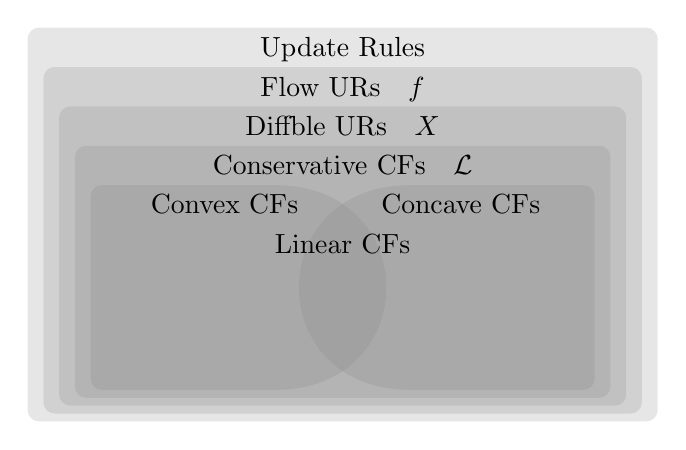
\begin{tikzpicture}
		\begin{scope}[fill=gray,fill opacity=0.2,rounded corners=4px]
			\fill (0,0) rectangle (8,5); \fill[] (0.2,0.1) rectangle (7.8,4.5); \fill[] (0.4,0.2) rectangle (7.6,4.0); \fill[] (0.6,0.3) rectangle (7.4,3.5); \fill (0.8,0.4) -- (0.8, 3.0) -- (3, 3.0)
			 	to[out=0,in=0,looseness=2] (3,0.4) --cycle; \fill (7.2,0.4) -- (7.2, 3.0) -- (5, 3.0)
			 	to[out=180,in=180,looseness=2] (5,0.4) --cycle; \end{scope}
		\begin{scope}[anchor=north]
			\node at (4.0, 5.0) {Update Rules};
			\node at (4.0, 4.5) {Flow URs~~~$f$};
			\node at (4.0, 4.0) {Diffble URs~~~$X$};
\node at (4.0, 3.5) {Conservative CFs~~~$\mathcal L$};
			\node at (2.5, 3.0) {Convex CFs};
			\node at (4.0, 2.5) {Linear CFs};
			\node at (5.5, 3.0) {Concave CFs};
		\end{scope}
	\end{tikzpicture}
	\caption{A map of different kinds of commitment functions and their representations.}
	\end{figure}
	}

\begin{figure*}
\centering
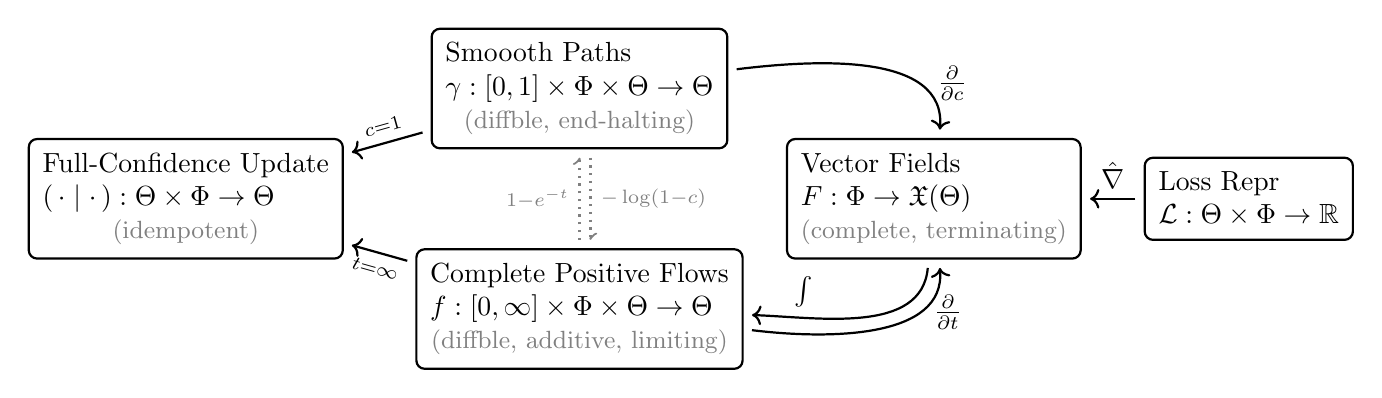
\begin{tikzpicture}
\begin{scope}[every node/.style={align=left,rounded corners=3,draw,thick,inner sep=5pt,anchor=center}]
	\node at (-5, 0) (fc) {Full-Confidence Update\\
		$(\,\cdot\mid \cdot\,) : \Theta \times \Phi \to \Theta$\\
			\small\hfill\color{gray}(idempotent)\hfill};
	\node at (0, -1.4)(flow) {Complete Positive Flows\\
		$f: [0,\infty] \times \Phi \times \Theta \to \Theta$\\
			\small\hfill\color{gray}(diffble, additive, limiting)\hfill};
	\node at (0, 1.4)(path) {Smoooth Paths\\ 
		$\gamma: [0,1] \times \Phi \times \Theta \to \Theta$\\
		\small\hfill\color{gray}(diffble, end-halting)\hfill};
	\node at (4.5, 0)(vfield) {Vector Fields \\
		$F : \Phi \to \mathfrak X(\Theta)$\\
		\small\hfill\color{gray}(complete, terminating)\hfill};
	\node at (8.5, 0) (loss) {Loss Repr \\
		$\mathcal L : \Theta \times \Phi \to \mathbb R$};
\end{scope}
	\draw[arr] (loss) to node[above]{$\hat\nabla$} (vfield);
\draw[arr] (path) to[out=7,in=85] 
		node[right=5pt,pos=0.7]{$\frac{\partial}{\partial c}$} (vfield);
	\draw[arr] (flow) to[out=-7,in=-85]
		node[right=3pt,pos=0.7]{$\frac{\partial}{\partial t}$} (vfield);
\draw[arr] (vfield) to[out=-95,in=-2] node[above=0pt,pos=0.75]
{$\int$}
		(flow);
\draw[arr] (path) to node[above, sloped]{$\scriptstyle c=1$} (fc);
	\draw[arr] (flow) to node[below,sloped]{$\scriptstyle t=\infty$}(fc);
	
	\draw[arr,-left to,dotted,gray] (path) edge[transform canvas={xshift=4pt}] 
		node[right]{$\scriptstyle-\log(1-c)$} (flow);
	\draw[arr,-left to,dotted,gray] (flow) edge
	 	node[left]{$\scriptstyle1-e^{-t}$}(path);
\end{tikzpicture}
\caption{Different representations of update functions, and the relationships they have with one another. 
Sections 3 and }\label{fig:map}
\end{figure*}


\begin{example}\label{ex:jugo}
Jugo is an impartial juror.
Like the other jurors, she has two buttons in front of her.
The button labeled $\mathsf G$ increases the probability 
of a guilty verdict, while the button labeled $\mathsf N$ increases
the probability of a not-guilty verdict. 
In more detail: let $J$ be the number of jurors, and $G_j(t)$ be
a variable that is equal to one if juror $j \in \{0, \ldots, J\}$
is pressing the $\mathsf G$ button at time $t$, and zero otherwise; 
symmetrically, let $N_j(t)$ indicate whether $j$ is pressing the $\mathsf N$ at 
time $t$. The belief state of this automated system is
represented by a single number $g \in [0,1]$.
If any individual juror presses the $\mathsf G$ button, 
the system evoves according to $\frac{\mathrm dg}{\mathrm dt} = (1-g)$;
we call this the \emph{vector field} associated with the $\mathsf G$ button.
The total effect of all buttons is then the sum of that of all buttons
across all vector fields, when they are active: 
\[
	\frac{\mathrm dg}{\mathrm dt} = 
	\sum_{j = 1}^J G_j(t) (1-g) 
		- g N_j(t)~,
                \]
%joe1                
%so that $g$ exponentially approahces $1$ when more $\mathsf G$ buttons
so that $g$ exponentially approaches $1$ when more $\mathsf G$ buttons
                are pressed than $\mathsf N$ buttons, 
%joe1
%and symmetricaly, exponentially approaches $0$ when more $\mathsf N$
and symmetrically, exponentially approaches $0$ when more $\mathsf N$
                buttons than $\mathsf G$ buttons are pressed. 
At the end of the trial, the defendant is convicted with probability
equal to the final value of $g$. 

Let $\phi$ represent a piece of evidence suggesting guilt, presented by the
prosecution from time $t_1$ to time $t_2$,
and suppose for now that only buttons labeled $\mathsf G$ are pressed
in this interval.
%joe1*: So pressing N has no effect on j's confidence in \phi?  
The system measures $j$'s confidence in $\phi$ by
\[
	w_j := \!\int_{t_1}^{t_2}\!\! G_j(t) \mathrm d t 
	= \text{ total time $j$ presses $\mathsf G$ during $\phi$,}
\]
%joe1*: not true; see my comment above
Note that $w_j = 0$ if and only if $j$ does not press any buttons,
which (a) indicates that $j$ does not trust the evidence $\phi$, 
and (b) communicates this fact to the system, by telling it to ignore 
the evidence. 
Note that this is an additive representation of confidence, since
pressing the button for four seconds, and then three more later, is
by definition the same as pressing it for seven. 
While the maximum possible confidence of $w_j$ is $(t_2 - t_1)$,
this system does not allow a juror to express \emph{full} confidence in $\phi$
because no finite amount of $\mathsf G$-pressing will result in a 
guilty verdict with probability one; it is always possible to increase
the value of $g$ through additional evidence. 

Altogether, the system's confidence in $\phi$ can be measured by
as the unique value $W$ for which
\begin{align*}
\int_{t_1}^{t_2} W (1-g(t)) \mathrm d t =
	 g(t_2) - g(t_1),
\end{align*}
which, so long as only $\mathsf G$ buttons are pressed, equals
$W := \sum_{j} w_j$, so this measure of confidence is additive 
across jurors as well as across time. 
%joe1*: appropriate for what?  
This is appropriate, since the jurors are independent and 
not communicating with each other.
As before, $W = 0$ if and only if no juror presses any buttons between times $t_1$ and $t_2$,
indicating zero trust leant to $\phi$. In such a case, the system ignores $\phi$ in updating its beliefs.
And just as no individual juror can send a full-confidence update to the system,
	the system cannot recieve a full-confidence from the jurors as a whole.

%joe1*: All this (indeed, the whole example) is completely
%inappropriate for the introduction.  You're introducing a whole bunc
%of new technical issues (the N button) and it's not clear how they
%relate to confidence as we originally introduced it. 	  
The picture gets significantly more complicated if we consider the possibility
that jurors might press the $\mathsf N$ button. For example, if $\phi$, which was intended
as evidence of guilt, has the effect of getting jurors to press $\mathsf N$, there is a sense
in which they have \emph{negative} confidence in $\phi$, since the belief update happened in the opposite direction of what $\phi$ represents; rather than \emph{no} trust, this is represents \emph{distrust}. 
Small negative updates are always possible except at the boundary of belief space, but in this paper, we focus almost entirely on positive confidence updates.

The introduction of the second button also uncovers a significant source of complexity:
unlike \cref{ex:prob-simple,ex:classifier,ex:shafer}, 
the order that evidence is presented matters, when there is more than one possible response to it.
Evidence presented later has a larger effect,
meaning that this system exhibits a recency bias.


Now consider a variant of this system that does
not trust all jurors equally; rather, it trusts each juror $j$
to a degree $\beta_j \in [0, \infty]$, and now $g$ evolves
according to
\[
	\frac{\mathrm dg}{\mathrm dt} = 
	\sum_{j = 1}^J \beta_j \Big( G_j(t) (1-g) 
		- g N_j(t) \Big).
\]
In this case, the system can be said to have trust $\beta_j$ in juror
$j$, since $j$'s buttons are ignored when $\beta_j = 0$. 
When $\beta_j = \infty$ (an expression of full confidence in $j$),
$g$ immediately jumps to 0 when $j$ presses 
$\mathsf N$, or to 1 if $j$ presses $\mathsf G$ (unless canceled by
another full-confidence juror pressing the opposite button).
If all jurors have full confidence, then the verdict of this system is
a majority vote at the last moment a button was pressed. 
Thus, the weights attached to weighted averages are (additive) expressions 
of confidence as well. 
\end{example}

\cref{ex:jugo} illustrates how a (sufficiently nice) vector field, 
	which is simpler than a smooth path for every starting point, is enough to define
an additive notion of confidence, via its integral curves.
It may seem strange to define confidence via a vector field, which does not mention confidence at all---but in a sense, it works because a vector field captures precisely everything about the update \emph{except} for the confidence. We do this formally in \cref{sec:vecrep}. 

In \cref{sec:loss-repr}, we demonstrate that it is typically possible to get an even more compact representation of the updating process, by representing the vector field implicitly as gradients of some ``loss function''.
To do this at full generality, we need to make sense of a gradient, which requires more structure, in the form of a Riemannian metric.  It turns out that, up to a multiplicative constant, there is a unique natural Riemannian metric on any parameterization of a probability distributions \cite{chentsov}; taking gradients with respect to this geometry, show how familiar loss functions on probability measures correspond to different standard notions of confidence in the other representations.

Once we have the formalism, fully in place, we give further examples of how confidence works in exponential families, in particular showing how Kallman gain and inverse variance can be viewed as confidence as well.



\commentout{
This general idea can be cleaned up by appeal to differential geometry.
Fix an input $\phi$.
Assuming that the update paths are differentiable in the degree of confidence at any initial beleifs, the collection of updates with infinitessimal confidence forms a complete vector field $X_\phi$ over the space of beliefs, whose integral curves are paths in belief space, parameterized by confidence $\beta \in [0,\infty]$.
We step through this more carefully in \cref{sec:field-repr}.

Finally, if our belief space is endowed with a Riemannian metric, so that we may take gradients, partial update functions may be specified by a loss.}













\commentout{
	\subsection{Other Conceptions of Confidence.}

	\textbf{Probability.}
Some people do use ``confidence'' to mean the same thing as probability. When they say they have low confidence in $\phi$, they mean that they think $\phi$ is unlikely.

	One of the biggest shortcomings of probability is its inability to represent a truly neutral attitude towards a proposition.
A value of $\frac12$ may be equally far from zero as it is from one, but is by no means a neutral assessment in all cases: hearing that your favored candidate has a 50\% chance of winning is big news if a win was previously thought to be inevitable.
	For this reason, telling someone the odds are 50/50 is quite different from saying you have no idea.
By contrast, zero confidence represents something truly neutral:
		a statement made with zero confidence does not stake out a claim, and
		a statement recieved with zero confidence does not affect the recipient's beliefs.
	Nevertheless, in some contexts, we will see that confidences correspond to to probabilities.

	\textit{Opacity.} To use a graphical metaphor, think of certainty as black or white.
	Probability describes shades of gray, while confidence describes opacity.
	If we are painting with black and start with a white canvas, there is a precise correspondence between the opacity and the resulting shade of gray.

	\textbf{Upper and Lower Probabilities.}
	Upper and lower probabilities can describe a neutral attitude towards a proposition, but they are not really a specification of trust, but rather a direct specification of a belief state.
	It isn't immediately clear how to use these representations of uncertainty to update, and they're a little too complex to function effectively as the primitive measure of trust that we're after.


	\textbf{Shafer's Weight of Evidence.}
	Shafer's ``weight of evidence'' is precisely the same concept we have in mind.
	Our analysis precsely reduces to his, in the setting where belief states are Belief functions (which generalize probabilities, but not, say, neural network weights), and observations are events.
Thus, this paper can be viewed as generalizing this concept to a broader class of settings, without requiring that one adopt Shafer's conception of a belief state or an observation.


	\textbf{Variance and Entropy.}
	The inverse of variance, sometimes known as precision,
		is also commonly used to measure confidence.
	If a sensor is unreliable and can give a range of answers, the variance of the estimate is a very common way of quantifying this reliablility.
	If measurements have zero variance, in some sense one has absolute confidence ($\top$) in the sensor. If measurements have infinite variance, then in some sense one has no confidence in the sensor, since individual samples convey no information about the true value of the quantity measured.
	As with probability, inverse variance will coincide with confidence in some settings; we will see how in \cref{sec:variance}.

	Entropy, like variance, is a standard way of measuring uncertainty, and in some settings, confidence coincides with entropy (see \cref{sec:entropy}).
	The assumption underlying both approaches is that there's some ``true'' value of the variable, and that the randomness is epsistemic (due to sensor errors) rather than aleotoric (inherrent in the quantity being measured).

	\textbf{Confidence Intervals and Error Bars.}
	Another notion of the word ``confidence'' comes from the term ``confidence interval''.
	This concept arises in settings involving a probability distribution $\Pr(X)$ over a metric space $X$, typically $X = \mathbb R$.
	A 95\% confidence interval is the (largest) ball containing 95\% of the probability, and its size is a geometric measurement of how .
	This intuition behind this reading of the word confidence is the same as
}
 
\section{A Formalism For Updating}

Throughout, we use $\Theta$ to refer to some space of possible belief states,
and $\Phi$ for a set of possible inputs. 
For example, a belief state $\theta \in \Theta$
might be probability distribution,
a Dempster-Shafer belief function, or
weights for a neural network,
while an input $\phi \in \Phi$ might be an event, or a sample from a dataset. 
Now, suppose we have some belief state $\theta$, and observe input $\phi$. 
How can we describe the processing of updating $\theta$, so as to obtain some $\theta'$ which takes $\phi$ into account?
To do so mathematically, we have to assume that it be captured in functional form.
\unskip\footnote{we can just as easily handle randomized updates;
	the point is simply that the update can be prescribed by an algorithm.}
\begin{CFaxioms}
	\item[\textbf{F}]
There exists a function $F : \Phi \times \Theta \to \Theta$ that,
		given prior beliefs $\theta$ and new information $\phi$, produces 
		posterior beliefs $\theta' = F(\phi, \theta)$.
\end{CFaxioms}

Given such a function $F$ and a statement $\phi$, we call $F_\phi = F(\phi, -) : \Theta \to \Theta$ an \emph{update}.
At face value, \textbf{F} seems quite reasonable:
aside from your beliefs and the new information, what more could your next belief state depend on?
We argue that one's \emph{confidence} in the new information $\phi$ is a third consideration,
worthy of special treatment.


 

Suppose
Since the purpose of $F$ is to \emph{fully} incorporate the new information into our beliefs
(and without a notion of confidence, we can't very well specify how much to incorporate),
then
two successive updates with the same information ought to have the same effect as a single one.
Intuitively, this is because if we have just updated our beliefs to be consistent with the information $\phi$, then a second observation of $\phi$ will require no further alterations of our belief state.
In this case, we call $F$ an \emph{update rule}, or more precisely, a \emph{$\Theta$-update rule on $\Phi$}, and insist that
\begin{CFaxioms}
	\item[\textbf{UR}] For all $\phi \in \Phi$, the update $F_\phi$ is
idempotent.
\end{CFaxioms}



Once $\Theta$, $\Phi$, and any implicit structure in them is specified, there is often a natural choice of update rule.
To illustrate, we now consider three different rules for different choices of $\Phi$.
In each case, the possible belief states $\Theta := \Delta W$ be the set of all probability distributions over a finie set $W = \{w_1, \ldots, w_n\}$ of ``possible worlds''.

\begin{enumerate}
	\item \textbf{Conditioning.}
	First, consider the case where observations are events, i.e., $\Phi := 2^W$.
Here, the appropriate rule seems to be conditioning:
	\[
	\begin{aligned}
		(-) \smash{\,\Big|\,} (\;\cdot\;) : \qquad 2^W &\to (\Delta W \to \Delta W) \\
A  &\mapsto (  ~\mu~~ \mapsto \mu \mid A ~),
\end{aligned}
\]
where the conditional measure $\mu\mid A$ is given by $(\mu \mid A)(B) = \ifrac{\mu(B \cap A)}{\mu(A)}$, provided $\mu(A) > 0$,
and otherwise is just equal to $\mu$.
	Observe:
	\begin{itemize}[nosep]
		\item Provided $\mu(A) > 0$, then $(\mu\mid A) \mid A = \mu \mid A$, so conditioning is an update rule.
		\item If $\mu(A \cap B) > 0$, then $(\mu \mid A) \mid B = \mu \mid (A \cap B) = (\mu \mid B) \mid A$, so the order that information is recieved does not matter, so long as that information is consistent with one's beliefs.
	\end{itemize}


	\item
	\textbf{Imaging.}
	A second example of an update rule is the ``imaging'' approach of David Lewis
	\parencite{lewis1976probabilities}.
Suppose that, for some set $\Phi$, that we already have a $W$-update rule
	$f : \Phi \to (W \to W)$, which we interpret as assigning, to each statement $\phi \in \Phi$ and $w \in W$, a unique world $f_\phi w \in W$ which is the world ``most similar to $w$, in which $\phi$ is true'' \parencite{gardenfors1979imaging}.
	In this case, idempotence of $f_\phi$ amounts to the (very reasonable) requirement that the world most similar to $f_\phi w$ in which $\phi$ is true, is $f_\phi w$ itself.
	From $f$, we can construct a $\Delta W$-update rule by
	\[
    	\begin{aligned}
    		F_\phi(\mu) &:=
    			f^{\sharp}(\mu)
= A \mapsto \mu(\{w : f(w) \in A\})
    	\end{aligned}
\]
	which intuitively moves the probability mass on each world $w$ to the $f_\phi w$, the closest world to $w$ in which $\phi$ is true.
And, since $f$ is idempotent, $F$ will be as well.


	\commentout{
	\item More generally, consider a measurable space $\mathcal W = (W, \mathcal A)$, where $W$ is a set and $\mathcal A$ is a $\sigma$-algebra over $W$, and let $\mathcal F \subset \mathcal A$ be closed under supersets in $\mathcal A$.


	\TODO[Properly Use Conditional Probability Measure, to define on all events]

	Conditioning a probability distribution $\mu \in \Delta\X$ on an event $A \in \mathcal A$ also makes sense in this more general measure-theoretic setting, at least so long as $\mu(A) > 0$, and is given by
$$
(\mu \mid A) (B) = \frac{\mu(B \cap A)}{\mu(A)}
	$$
	}


	\item \textbf{Jeffrey's Rule.}
Next, consider a more general form of observation, in which observations themselves are probabilities.
Formally, suppose $\Phi$ consists of distributions $\pi(X)$,
where $X : W \to S$ is a random variable,
and $\pi \in \Delta S$ is a distribution over the possible values that $X$ can take.
	Jeffrey's rule, given by
	\begin{align*}
\mathrm{J}_{\pi(\mskip-2muX\mskip-2mu)}
		(\mu) &:= \sum_{x \in S} \pi(X{=}x) \;  \mu \big|
            X{=}x
\\
			&= A \mapsto \sum_{x \in S} \pi(X{=}x)\, \mu( A \mid X \!= x)
	\end{align*}

	When $\pi(X) = \delta_x$ is a point mass $X=x$, then Jeffrey's Rule simply conditions on the event $X = x$.
For this reason, Jeffrey's Rule is sometimes often thought of as a generalization of conditioning that admits for less that complete certainty (i.e., ``low-confidence'' updates), but as we will see, it instead is perhaps better thought of as a high-confidence update on a more expresive class of observations.

	Note that if $\mu' := J_{\pi(X)}(\mu)$ is the result of applying Jeffrey's rule to $\pi(X)$ and $\mu$,
then $\mu'(X) = \pi(X)$, so $\pi(X)$ has been fully incorporated into $\mu'$, and the old beliefs $\mu(X)$ about $X$ have been completely destroyed by the update.
\end{enumerate}
 
\section{Fractional Updates, and the
    Flow Representations}


If we take a step back, fully incorporating information is really quite extreme.
An agent that updates with conditioning for instance, is forever committed to fully believing $A$, and consequently, learns nothing from observing $A$ agin in the future.
Clearly humans are not like this.
Similarly, artificial neural networks are trained with many incremental updates, and cycle through training data more than once.
Indeed, this is one biggest differences between modern machine learning techniques and  older rule-based ones: modern algorithms update parameters little-by-little, rather than fully incorporating input information.
How shall we alter our picture to account for less extreme belief alterations, in which information is only partially incorporated?
This is where confidence comes in.








Let $\confdom$ be the set of possible confidences, which, for now, we will take to be the interval $[0, 1]$.
We are now in a position to take confidence into account in our updates.
As before, our first axiom is that we can capture the updating process in functional form.

\begin{CFaxioms}
	\item[CF0]
	There exists some function
\[
		F : \confdom \to ( \Phi \to ( \Theta \to \Theta) )
	\]
	which, given a confidence and new information $\phi$, in addition to a prior belief state $\theta$, produces the belief state $F^c_\phi\theta$ that corresponds to the result of observing $\phi$ in state $\theta$. \label[CFaxiomsi]{ax:funcform}
\end{CFaxioms}



Historically speaking, \cref{ax:funcform} has not proved as anodyne as it looks.
Some might object that it's not possible to write such a function that is appropriate in all circumstances.
For example, Shafer argues for Dempster's rule of combination as a way of incorporating information, but is very careful to emphasize that it ought to be used only on \emph{independent} information, for reasons illustrated below.



\begin{example}\label{ex:dupl}
	You have initial belief state $\theta_0$.
	Now, someone comes up to you and tells you that $\phi$ is true, a statement
		that you trust to some intermediate degree of confidence $c \notin\{ \bot, \top\}$.
	So, in accordance with \Cref{ax:funcform}, you use $F$ to transform your beliefs, partially incorporating the information to arrive at some belief state $\theta_1 := F^c_\phi(\theta_0)$.
	Immediately afterwards, your friend repeats what they just said: $\phi$ is true.
	Your confidence in the statement remains the same, and so according to
	\Cref{ax:funcform}, you again update your beliefs, arriving at $\theta_2 := F^c_\phi(\theta_1)$.
	Except in very special circumstances (e.g., you already know that $\phi$ is true, or $c \in \{\bot,\top\}$), typically $\theta_2$.
	And yet, it seems your your attitude towards $\phi$ ought to be the same whether you've heard it twice or only once.
\end{example}


Now, it's important to mention that we're not quite in the same position as Shafer.
Shafer was prescribing a concrete representation of $\Theta$ (a belief function) and a concrete update rule $F$ (Dempster's rule of combination), and so he needed to defend these choices.
We only need to defend something much more modest: we only need to defend the assumption that, if $\Theta$ and $\Phi$ properly model the relevant aspects of the scenario at hand, then there exists \emph{some} function $F$ which performs updates appropriately.
Descriptively speaking, we're also in good shape: for synthetic agents, it suffices to point out that learning algorithms represent functions, which given a state, an input, and a number of iterations (confidence), produce an output.
And, supposing that $\Theta$, $\Phi$, and $\confdom$ all capture the relevant respective aspects of a human's belief state, input information, and attitude towards it, how could it be that a human does otherwise?
In any case, keeping \cref{ex:dupl} in mind, here are three ways to proceed.

\begin{enumerate}[label={\textbf{I\arabic*.}},ref={I\arabic*}]
	\item \textbf{Accept Severe Limiations.} \label{approach:assume}
	Like Shafer, we could be careful
to claim nothing about the belief updating process except in the (unusual) case where
	information recieved is independent.
This would be a severe limiation to the theory, and much less necessary than it was for Shafer.
	Imagine that we are writing code that describes how a synthetic agent updates its beliefs. Shafer's approach is to package any such code with a warning against running it unless assured that observations will always be independent.
	But independece is notoriously difficult to establish; are we to simply accept that the code will not behave correctly in any realistic scenario?


	In practice, many theoretical properties of standard statistical learning algorithms are heavily dependent on indepencence assumptions (most commonly, that one recieves independent, identically distributed samples).
This warning label not seem to keep them from being applied in settings where practitioners readily admit samples are not really independent at all---nor indeed performing well emperically in those settings \parencite{???}.




	\item \textbf{Appropriately Enrich Domains.}\label{approach:enrich}
In \cref{ex:dupl}, it seems obvious that we ought to ignore the second copy of the information, because it has already been accounted for.
	However, this intuition is highly contingent on the implicit supposition that we \emph{know} the second input to be a replica of the first.
	Were we ignorant to the nature of the second piece of information, perhaps it would not be so unreasonable to incroproate it again, even without a proof of independence.
So, if we would like our agent to make the same decisions that we did, it seems only fair to give it access to the knowledge that we needed to get there.
	One way of doing this is to extend the belief state so that it also tracks what information has been incorporated.


	For \cref{ex:dupl} to work, it is critical that we are able to discern that the two inputs were identical.
	As a result, it seems that the relevant description of the input information was not just $\phi$, but a pair $(\phi, \mathit{id})$ that also a description of its identity.
	It is also critical that we remember the identity of previously incorporated information, so we would also be better off with a belief space $\Theta$ reflects this.
	With these two modifications, any \cofunc\ can be straightforwardly modified to avoid the issue in \Cref{ex:dupl}.


	We submit that it is always possible to enrich the space of beliefs and observations in this way to track the relevant information, to resolve the issue.
	With a few more assumptions later on, we will be able to formalize the construction we just alluded to (\cref{ex:dupl-enriched}).

	\item \textbf{An Incremental Interpretation of Confidence.}
		\label{approach:interperet}
	Finally, we can get around the issue by interpreting a confidence $c \in \confdom$ not as an absolute measurement of confidence, but rather an incremental one.  This means viewing $c \in \confdom$ as the degree of \emph{additional} confidence we have in $\phi$, beyond whatever we have already incorporated into our beliefs.

This proposal might be concerning.
One might worry that it's harder to make sense of ``incremental confidence'' than an absolute notion.
	How ought we to numerically describe the confidence of an update?
	Suddenly this becomes much more subjective, for to assign a number, not only must we describe how much trust we have in the new information, but we must also take history or current belief state into account.
	Furthermore, the words ``incremental'' and ``additional'' suggest that we will need a formal description of how to aggregate confidences---the very concept of which we will need to defend.


	Even modulo these concerns, the incremental interpretation still leaves us in a strictly better place than we were before.
To begin, in situations where inputs are independent (i.e., the only cases where we would have been allowed to apply the \cofunc\ according to \cref{approach:assume}), the two notions coincide.
	More explicitly: if the new information $\phi$ is indepenendent of everything we've previously seen, then an absolute measurement of our confidence in it is no different from a measrurement of how much we ought to increment it from having no confidence.
	Already, though, we can do more.
	In the situation described by \cref{ex:dupl}, for instance,
	the second utterance induce no \emph{additional} confidence ($\bot$), and so applying $F$ with no confidence clearly gives the desired result of ignoring the new information (per \cref{ax:zero}).
And even in general, the prospect of having to numerically estimate a fuzzy quantity seems more promising than red tape requiring that $F$ only be used (in good conscience) on independent information.


\end{enumerate}





Given a confidence $c \in \confdom$ and a statement $\phi \in \Phi$, we write
$F^c_\phi : \Theta \to \Theta$
for the update prescribed by the \cofunc\ $F$.
Furthermore, we will insist that \cofunc s respect our interpretation of confidence at the two extremes.
\begin{CFaxioms}
\item
For all $\theta \in \Theta$ and $\phi \in \Phi$, $F^{\bot}_\phi(\theta) = \theta$.
\hfill \textbf{(neutrality)} \label{ax:zero}
\item
For all $\phi$,
$F^\top_\phi : \Theta \to \Theta$
		is an idempotent update.\\
		Equivalently, $F^\top: \Phi \to (\Theta \to \Theta)$ is an update rule.
\hfill \textbf{(certainty)} \label{ax:idemp}\\
		We call $F$ a \emph{refinement} of the update rule $F^\top$.
\end{CFaxioms}
\Cref{ax:zero} captures the intuition that we should ignore information in which we have no confidence, while \cref{ax:idemp} formalizes the intuition that a full-confidence updates act as we imagined.
At this point, we would like to point out that those who find \cref{ax:zero} reasonable have implicitly either accepted either \cref{approach:assume} or \cref{approach:interperet}.

\begin{example}
	Suppose you first hear $\phi$ from a partially trusted source, and incroproate it into your beliefs appropriately.
	Then, the same source sends you a second message, which is obviously spam.
	In an absolute sense, you now have no confidence ($\bot$) in anything this source tells you, including (in retrospect) both messages.
	It seems appropriate to excise $\phi$ from your belief state in response, rather than leaving your belief state unchanged, as \cref{ax:zero} would prescribe.

	Note that in this scenario, while it seems that we ultimately have no confidence in $\phi$, it does not seem to be the case that we have no incremental confidence in $\phi$.
	Rather, the incremental confidence seems to be the inverse of the original confidence.
\end{example}

>From this point forward, we use the incremental interpretation of confidence, with the understanding that
all of our results also admit a more conservative reading, in which confidence is measured absolutely, and also all applications of the function $F$ are independent. 







\begin{phaseout}
and so for most of this paper, we take $\confdom := \Rplus$ to be the group of extended nonnegative real numbers under addition.
With this choice of confidence domain, \cref{ax:additivity} begins to have more bite, although, as we will see, the effect is more to pin down a coherent system of measurement, and does not appear to restrict modeling expressivness.



Here are some more abstract examples of \cofunc s, with confidence domain
$\confdom := \mathbb R_+$.
\begin{enumerate}
\item
Once again, suppose $W$ is a finite set,
$\Theta := \Delta W$, and $\Phi := 2^W$.
Here are two natural \cofunc s for this scenario, both of which are refinements of conditioning.
\begin{itemize}
	\item
	$\displaystyle
		(F1^c_A \mu)(B) = (1-e^{-c}) \mu(B|A) +  e^{-c} \mu(B)
	$
	\item
	$\displaystyle
		(F2^c_A \mu)(B) \propto \mu(B|A)^{(1-e^{-c})} \mu(B)^{e^{-c}}
	$
\end{itemize}
The first \cofunc, $F1$, linearly interpolates between the result of ignoring the information contained in the event $A$ (i.e., leaving the belief state $\mu$ unchanged) and conditioning on $A$.
By contrast, $F2$ does a similar interpolation, but multiplicatively.

\item
Suppose that $\Theta$ is the set of possible parameter settings for a neural network, which aims to predict an element of $Y \subset \mathbb R^{m}$ given an in put from $X \in \mathbb R^{n}$.
So, for each $\theta \in \Theta$, we have a function $f_\theta : X \to Y$, and for fixed $x \in X$, the function $\theta \mapsto f_\theta(x) : \Theta$ is differentiable.






\item
Again consider a finite set $W$ and suppose $\Theta$ consists of all Dempster-Shafer belief functions
\end{enumerate}







We are particularly interested in the setting where $\Theta$ parameterizes a family of probaility distributions.
To that end, suppose that $\X = (X, \mathcal A)$ be a measurable space, so that $X$ is a set and $\mathcal A$ be a $\sigma$-algebra over it, let $\Delta \X$ denote the set of probability measures over $\X$,
and keep in the back of our heads an indexed family
$
	\mathcal P =
	\{ p_\theta \in\Delta\X \mid \theta \in \Theta \}
$ of probability distributions.
\end{phaseout}

 
\section{Differentiable Updates, and their
    Vector Field Representation}

Confidence is meant to interpolate between fully incorporating information and ignoring it.
Such an interpolation becomes more useful if it is continuous, and more useful still if it is differentiable.
Next, we present two variants of a differentiability axiom, depending on the structure one has in hand. 

\begin{CFaxioms}
	\item \label{ax:diffble}
	\begin{enumerate}
	\item $\Theta$ has a manifold structures, and
		for all $\theta$ and $\phi$, the function $\beta \mapsto F^{\beta}_\phi(\theta) : \confdom \to \Theta$
		is continuously differentiable at $\beta = \bot$. \item 
		$\Theta$ parameterizes a family of probabilities over $(\X, \mathcal A)$,
		via $\{ \Pr_\theta \}_{\theta \in \Theta}$.
for all $\theta \in \Theta$, $\phi \in \Phi$, and  $A \in \mathcal A$,
		the function $\beta \mapsto \Pr_{F^{\beta}_\phi(\theta)}(A)
		: \confdom \to \mathbb [0,1]$ is
		continuously differentiable at $\beta=\bot$. 
\label{ax:diffble2}
	\end{enumerate}
	\hfill \textbf{(differentiability)}
\end{CFaxioms}



If $\Theta$ is a differentiable manifold and $\Pr: \Theta \to \Delta\X$ is a differentiable map, then the second follows from the first. 
It's simpler to assume that $\Theta$ carries a differentiable structure, so we will assume this when possible.


When we have $\confdom := \Rplus$,

\TODO


\begin{CFaxioms}
	\item For all $\beta_1, \beta_2 \in \Rplus$,~
$F^{\beta_1}_\phi \circ F^{\beta_2}_\phi = F^{\beta_1 + \beta_2}_\phi$
\hfill \textbf{(additivity)} \label{ax:additivity}
\end{CFaxioms}




\begin{prop}
	If $F$ is a differentiable \cofunc\ with confidence domain $\Rplus$,then there is a unique update rule $G$ with the same confidence domain, that behaves approximately like $F$ for small increments of confidence, and is also additive (\cref{ax:additivity}).
\end{prop}





\label{sec:vecrep}
For a smooth manifold $M$
(such as the space $\Delta \X$ of distributions over $\X$),
and a point $p \in M$, we follow convention by writing $T_p M$ for the tangent space to $M$ at point $p$ \parencite{lee2013smooth}, and $TM := \sum_{p \in M} T_p M$ for the full tangent bundle over $M$.
A vector field over $M$ is a smooth map $\mat v : M \to T M$ assigning a tangent vector $\mat v(p) \in T_p M$, to every point $p \in M$.


\begin{theorem}
Every update rule $F : \Phi \times \mathbb R \to (\Theta  \to \Theta)$
satisfying \cref{ax:zero,ax:additivity,ax:diffble} corresponds to a unique
$\Phi$-indexed collection of vector fields
    $F' : \Phi \times \Theta \to T\Theta$
\end{theorem}


In the language of 

\begin{coro}\label{thm:vecrep}
There is a bijective correspondence between udpate rules satisfying \cref{ax:zero,ax:additivity,ax:diffble} and $\Phi$-indexed collections of \textbf{complete} vector fields.
\end{coro}


We call $F'$ the \emph{vector field representation} of a differentiable update rule $F$.

This vector field representation of a commitment function captures everything except the confidence itself. 

One defining feature of vector fields is closure under linear
combination.  Because they are in natural correspondance with differentiable additive update rules, update rules also inherit this structure.

In particular, given \cofunc s $F, G : \mathbb R \to \Theta$, we can define
$F \oplus G$ via the vector field $(F \oplus G)' = F' + G'$.

\begin{wip}
\textbf{Interaction With Certainty Axioms.}

\TODO[TODO: prove impossible to individually they satisfy certainty, but not together.]
\end{wip}

\begin{defn}
For an assertion language $\Phi$, let $\ext\Phi$ denote
the space of weighted formal sums of elements of $\Phi$.
\end{defn}

\begin{prop}
Every  update rule $F$ on $\Phi$, can be naturally extended to an update rule
$\bar F$ on $\ext\Phi$
via the total vector field
\[
\bar F'_{\textstyle\sum_i a_i \phi_i} ( \theta ) := \sum_{i} a_i F'_{\phi_i}(\theta).
\]
\end{prop}

If $\Phi$ is itself a measurable space, we can extend this further:
Every  update rule $F$ on $\Phi$, can be naturally extended to an update rule $\bar F$ on the space $\mathcal M(\Phi)$ of measures over $\Phi$, via
\[
\bar F'_{\beta(\Phi)}( \theta ) := \int_{\Phi} F'_\phi(\theta) \mathrm d\beta.
\]





\subsection{Linear Update Rules}



There are many definitions of linear update rules:
\begin{defn}\label{ax:linear}
Let $F$ be a differentiable update rule on $\Theta$. We say that $F$ is \textellipsis
\begin{itemize}
\item \emph{linear} if $\Theta$ is a vector space over $\mathbb R$, and the
vector field $F'_\phi$ is a linear operator, i.e., for all $a, b \in \mathbb R$, we have that
\[ F'_\phi(a \theta_1 + b \theta_2) = a F'_\phi(\theta_1) + b F'_\phi(\theta_2). \]

\item \emph{cvx-linear} if $\Theta \subset \mathbb R^n$ is a convex set, and, for all $a \in [0,1]$, we have that
\[ F'_\phi(a \theta_1 + (1-a) \theta_2) = a F'_\phi(\theta_1) + (1-a) F'_\phi(\theta_2). \]

\item \emph{$\mathcal L$-cvx-linear} if $\Theta \subset \mathbb R^n$ and $F$ is an optimizing update rule with a loss representation $\mathcal L$ linear in its first argument, i.e.,
\[
    \mathcal L(a \theta_1 + (1-a) \theta_2, \varphi) = a \mathcal L(\theta_1, \varphi) + (1-a) \mathcal L(\theta_2, \theta).
\]
\end{itemize}
\end{defn}

\begin{prop}
If $F$ is a $\mathcal L$-cvx-linear, then it is also cvx-linear.
\end{prop}

In fact, the first condition is much stronger;
\begin{prop}
if $F$ is a nontrivial $\mathcal L$-cvx-linear optimizing UR, then $\Theta$ equals cone generated by  the rays $\{ F'_\varphi\theta : \theta \in \Theta, \varphi \in \Phi \}$. In particular, if there is some $\theta$ such that $0$ is in the interior of the convex hull $\mathrm{conv}(\{F'_\phi\theta\}_{\phi \in \Phi})$, then $\Theta = \mathbb R^n$.
\end{prop}



\begin{prop}
Every linear update rule is of the form
$
    F^{\beta}_\phi(\theta) =  \theta^{T} \exp(\beta V)
$,
where $\exp(\beta V)$ is the matrix exponential.\footnote{Concretely, if $V = U^T \mathrm{Diag}(\lambda_1, \ldots \lambda_n) U$ is an eigendecomposition of $V$, then $\exp(V) = U^T \mathrm{Diag}(e^{\beta\lambda_1}, \ldots e^{\beta\lambda_n}) U$.}
\end{prop}

\begin{prop}
A linear update rule $F$ is commutative iff, for every pair of statements  $\phi, \phi' \in \Phi$, the
matrices $V_\phi$ and $V_{\phi'}$ commute.
\end{prop}
 
\section{Optimizing Updates, and their
    Loss Represntation}
Suppose we have:
\begin{enumerate}[nosep]
	\item A differentiable loss function $\mathcal L : \Theta \times \Phi  \to \mathbb R$, which intuitively measures the ``incompatibility'' between a belief state $\theta$ and an assertion $\varphi$, and
	\item
A way of taking the gradient of ${\cal L}$ with respect to $\theta$,\footnote{
			such as a tangent-cotangent isomorphism $(-)^\sharp : T^*_p\Theta \to T_p \Theta$, perhaps coming from an affine connection, in turn perhaps coming from a Riemmannian metric.}
        so as to obtain a vector field on $\Theta$ which optimizes $\mathcal L.$
\end{enumerate}
\def\GD#1{\mathtt{GF}[#1]}
\def\NGD#1{\mathtt{NGF}[#1]}

Then we can define an update rule $\GD {\cal L}$ that reduces inconsistency by gradient flow (the continuous limit of gradient descent). Concretely, such an update rule has a vector field:
\[
	\GD {\cal L}'_\phi(\theta) = - \nabla_\theta {\cal L}(\theta,\phi).
\]


\begin{prop}
	An update rule $F$ on a Riemannian manifold $\Theta$ is optimizing update rule if and only if $(F')^\flat$ is a conservative co-vector field.
	\cite[Prop 11.40]{lee2013smooth}
\end{prop}



\begin{example}[Weighted Average]
	\begin{align*}
		\Theta = \mathbb R^n \times (\mathbb R_{> 0} \cup \{\infty\});
		\qquad
		\Phi = \mathbb R^n \end{align*}
	A belief state $(\mat x,w) \in \Theta$ consists a current estimate $\mat x$ of the quantity of interest, and a weight $w$ of the total internal confidence in the estimate.

	Updating proceeds by taking a weighted average of the previous estimate and the new input, weighted by their respective confidences, which is captured by:
	\begin{align*}
		F^\beta_{\mat y}(\mat x, w) &=  \left( \frac{ w \mat x + \beta \mat y}{w + \beta} , w + \beta \right)
		~~\text{and}~~
		F^{\beta}_{\mat y}(\mat x, \infty) = (\mat x, \infty)
	\end{align*}
	It is additive, since
	\begin{align*}
		&F^{\beta_2}_{\mat y} \circ F^{\beta_1}_{\mat y}(\mat x, w) \\
		&= \left( \frac{ (w + \beta_1) \frac{ w \mat x + \beta_1 \mat y}{w + \beta_1} + \beta_2 \mat y}{(w + \beta_1) + \beta_2}, (w  + \beta_1) + \beta_2 \right) \\
		&= \left( \frac{  w \mat x + (\beta_1 + \beta_2) \mat y}{w + (\beta_1 + \beta_2)}, w  + (\beta_1 + \beta_2)\right)
		= F^{\beta_1 + \beta_2}_{\mat y}(\mat x, w).
	\end{align*}
	And it is clearly differentiable, with a simple calculation revealing that
	$ F'_{\mat y}(\mat x, w) = \left( \frac{\mat y - \mat x}{w}, 1\right) $.

	Observations:
	\begin{itemize}
		\item The update rule cannot be extended differentiably to states $\theta = (\mat x, w)$ with $w = 0$.
			Intuitively, we need to have some estimate with positive confidence to update beliefs in a differentiable way.
			This is related to the fact that plain emperical risk minimization (ERM) is unstable, but stable with even a small amount of regularization.
\item The certainties are given by
		\[
			\lim_{\beta \to \infty} F^{\beta}_{\mat y}(\mat x, w) = (\mat y, \infty)
		\]
\item $F$ is commutative, invertible, and symmetric with respect to permutation of the dimensions, but it is not conservative: if we had $U(\mat x, w, \mat y)$ twice differentiable such that $\nabla_{\mat x, w} U = F'$, then we would have
        \begin{align*}
        \frac{\partial^2}{\partial w \partial x_i} U &=
			\frac\partial{\partial w} \frac{y_i - x_i}{w} = \frac{x_i - y_i}{w^2},\quad\text{but}
            \\
		\frac{\partial^2}{\partial x_1 \partial w} U
			&= \frac\partial{\partial x_i} 1 = 0    
        \end{align*}
		violating Clairaut's theorem on equality of mixed partials.
		Therefore, $F$ is not an optimizing update rule.
	\end{itemize}
\end{example}

\textbf{Natural Gradients for Probability Distributions.}
When $\Theta$ parameterizes a family of probability distributions, via some $\Pr : \Theta \to \Delta \X$, there is a particularly natural metric on $\Theta$, called the Fisher information metric.
This metric is the unique one on $\Theta$ that is
independent of the representation of $\X$ \parencite{chentsov}, in the following sense.
If there are cpds $p(Y|X)$ and $q(X|Y)$ such that, for all $\theta \in \Theta$,
the distribution $\Pr_{\theta}(X)$ is unchanged after converting to $Y$ and back again $X$ (via $p$ and $q$ respectively), as depicted by the following commutative diagram,
\[
\begin{tikzcd}
		\Theta \ar[r,"\Pr"]\ar[d,"\Pr"']
& X \\
		X \ar[r,"p"'] & Y \ar[u, "q"']
	\end{tikzcd}
\]
then clearly the family $\Pr(Y|\Theta) := p\,\circ\,\Pr_{\theta}$ carries the same information about the parameters (and in particular how best to update them) as $\Pr_\theta$.
Chentsov's theorem says, that, up to a multaplicative constant, the Fisher information metric is the only metric on $\Theta$, as a function of the parameterization $\Pr$, which gives identical geometry in both cases.



At each point $\Theta$, the components of the Riemannian metric form a matrix---in this case, the Fisher information matrix $\mathcal I(\theta)$---which allow us to now compute the gradient in the natural geometry from the coordinate derivatives as
\[
	\NGD {\cal L}'_\phi (\theta) = - \hat \nabla_\theta \mathcal L(\theta,\phi)
= \mathcal I(\theta)^{\dagger}  \nabla \mathcal L(\theta, \phi)
\]
where $ \mathcal I(\theta)^{\dagger} $ denotes the Moore-Penrose psuedoinverse of the matrix $ \mathcal I(\theta)$,
and $\nabla \mathcal L$ is the gradient for the euclidean metric i.e., the vector of partials $[\frac{\partial \mathcal L}{\partial \theta_1}, \ldots, \frac{\partial \mathcal L}{\partial \theta_n}]^{\mathsf T}$.




\subsubsection{Expected Utility Maximization Update Rules}





\def\Bolz#1{\mathrm{Bolz}[#1]}




Suppose, for each $\phi \in \Phi$, we have a utility function $U_\phi : X \to \mathbb R$ on the underlying set $X$.
We can use this to define an update rule

\begin{align*}
	\Bolz U &: (\mathbb R \times \Phi) \to \Delta\X \to \Delta\X \\
	\Bolz U^\beta_\varphi(\mu)
		&:\propto
			\mu \exp(-\beta U_\phi) \\
		&= A \mapsto \frac
			1{\Ex_{\mu} [ \exp(-\beta U_\phi)]}
			{\int \exp(-\beta U_\phi) \mathbbm 1_A \mathrm d\mu }
\end{align*}

\begin{prop}
	Bolzmann Update Rules are additive, zero, differentiable, invertable, and commutative.
\end{prop}

\begin{lproof}
	\textbf{Commutativity.}
	For some normalization factors $Z, Z', Z''$, we have:
	\begin{align*}
		 F^\beta_\phi( F^{\beta'}_{\phi'}(\mu))
		 &= F^\beta_\phi \Big( \frac{1}{Z} \,\mu\, \exp(- \beta' c_{\phi'}) \Big) \\
		 &= \frac{1}{Z'} \frac{1}{Z} \,\mu\, \exp(- \beta' c_{\phi'}) \exp(- \beta c_{\phi}) \\
		 &= \frac{1}{Z''} \,\mu\, \exp(-\beta' c_{\phi'} - \beta c_\phi)
	\end{align*}
	which is the same expression when we exchange $(\phi, \beta)$ and $(\phi', \beta')$.
\end{lproof}

Note that this is true even for costs generated by asymmetric distances $c_{\{y\}}(x) = d(y, x) \ne d(x,y) = c_{\{x\}}(a)$.


\begin{remark}
Regarding $U_\varphi : \X \to \mathbb R$ as a potential energy over $X$,
	$\Bolz U^\beta_\varphi(\Unif)$ is the Boltzmann distribution at inverse temperature (thermodynamic coldness) $\beta$
In the thermodynamic analogy, as temperature decreases, one becomes more certain that particles are in their most favorable states.
\end{remark}


The certainties of $\Bolz U$ are the minimizers of $U$.





\begin{wip}
As a reminder, we have $\Theta = \Delta \X$, and suppose we have $c : X \times \Phi \to \mathbb R$.
	Suppose $U(\theta, \varphi) = \Ex_\theta[ c_\varphi ]$ (linearity, \cref{ax:linear}).
	Then
	$(\mathrm{Boltz}\;U)'_\varphi \theta = \theta(\Ex_\theta[c_\varphi] - c_\varphi),
	$while
	\begin{align*}
		 (\mathtt{GD}\; U)'_\varphi \theta &=
			 - \nabla_{\theta} \Ex\nolimits_\theta [ c_\varphi ]
			 \\ &= - c_\varphi
.
	\end{align*}
	This second expression, though, doesn't seem quite right --- it isn't even a tangent vector to the probability simplex, since its components don't sum to zero.
	This issue is in our naive computation of the gradient.
	We have computed the collection of partial derivatives $\frac{\partial}{\partial \theta_i} ( \theta \cdot  c_\varphi) = (c_\varphi)_i$,
	which is technically  co-vector field, not a vector field.\footnote{it acts on a vector field $V$ by $ -c_\varphi ( V ) = - V(c_\varphi)$.}

	For simplicity, suppose that $X = \{1, \ldots, n\}$, in the discussion that follows.
	If our parameter space were all of $\mathbb R^n$, we could simply collect these terms and take a transpose, to get
	\[
		\nabla_\theta \Ex_{\theta}[c_\varphi]
	\]
	There are two ways to proceed from here.
	The first makes use of manifold theory: for each point $p \in \Delta X$, begin by identifing a neighborhood $U \ni p$ with an open subset of $\mathbb R^{(n-1)}$, and define an inner product (a metric tensor) $g_p(\cdot, \cdot)$ on tangent vectors $v \in T_p\Delta X$, making $\Delta\X$ into a Riemannian Manifold, and then compute the gradient in the standard way, using the inverse of the metric tensor $g$ in order to convert covectors to vectors in a natural way.

The second, which is computationally simpler, is to take the metric induced by an embedding in Euclidean space.
	This approach is equally general, because Nash's Theorem \parencite{nash1956imbedding} tells us that any $n$-dimensional Riemannian manifold may be isometrically embeded in $\mathbb R^{2n+1}$.



\end{wip}

\begin{prop}
The associated vector field is given by
$
(\mathrm{Boltz}\,U)'_\varphi p = p (\Ex_p[U_\varphi] - U_\varphi )
	$.
\end{prop}
\begin{lproof}
	Let $f(X) := \exp(-\beta U(X,\varphi))$, and $g(X) := U(X,\varphi)$.
	\begin{align*}
		\mathrm{Boltz}'_\varphi\theta &= \frac{\partial}{\partial \beta} \mathrm{Boltz}^\beta_\varphi(p) \Big|_{\beta=0} \\
	\intertext{\TODO[TODO: finish typesetting algebra]}
		&= x \mapsto
			p(x) \frac{f(x)}{\Ex_p[f]}
				\left(\Ex_p\left[ \frac{f}{\Ex_{p}[f]} g\right] - g(x) \right)
\Big|_{\beta=0}
				\\
		&= \frac{pf}{\Ex_p[f]^2}
			\left(\Ex\nolimits_p\left[ f g\right] - g \Ex\nolimits_{p}[f] \right)
			\Big|_{\beta=0} \\
		&= x \mapsto p(x) (\Ex\nolimits_p[g] - g(x)) &
			\text{since $f(X) = 1$ when $\beta=0$}
	\end{align*}
	As a sanity check, note that the sum over all components is
	\[ \sum_{x \in X} ((\mathrm{Boltz}\,U)'_\varphi\, \theta)_x
		 = \sum_{x \in X} p(x) (\Ex\nolimits_p[g] - g(x))
		 = \Ex\nolimits_p[ \Ex\nolimits_p [ g ]] - \Ex\nolimits_p [g] = 0,
	 \]
	 so indeed it lies within the tangent space.
\end{lproof}


\begin{prop}
	The optimizing update rules for $\Theta = \Delta X$ whose loss represntation is linear (i.e., an expected utility), are precisely the Bolzmann update rules.
	In particular, the Bolzmann update rule with potential $U(X)$ is the natural gradient flow update rule for expected value of $U$, i.e.,
	\(
		\Bolz U =
		\NGD{\mu\mapsto\Ex_\mu U} .
	\)
\end{prop}


\begin{example}[Gaussian NGD]\label{gauss-ngd}
	Consider the case where $\Theta  = \{ (\mu, \sigma^2) \in \mathbb R \times \mathbb R_+ \}$ is the half-space of parameters to a Gaussian over some real variable $X$, and $\Phi \cong \mathbb R$ consists of possible observations of $X$.

	One natural loss function is negative log likelihood (differential surprisal) of the observation $x$ according to your belief state $\theta = (\mu, \sigma^2)$:
	\begin{align*}
		&\mathcal L(x, \mu, \sigma^2) = - \log \mathcal N(x \mid \mu, \sigma^2) 
        = \frac12 \log 2\pi\sigma^2  + \frac12 \left(\frac{x-\mu}{\sigma}\right)^2 \\
        &\quad=
		\aar*{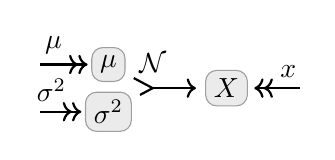
\begin{tikzpicture}[center base]
			\node[dpad0](X) at (0,0){$X$};
\draw[arr2, <<-] (X) to node[above,pos=0.7]{$x$} ++(1.0,0);
\node[dpad0](m) at (-1.5, 0.3) {$\mu$};
			\node[dpad0](s2) at (-1.5, -0.3) {$\sigma^2$};
			\mergearr{m}{s2}{X};
			\node[above=2pt of center-ms2X](N){$\mathcal N$};
			\draw[arr1, <<-] (m) to node[above, pos=0.7]{$\mu$} +(-0.9,0);
			\draw[arr1, <<-] (s2) to node[above, pos=0.7]{$\sigma^2$} +(-0.9,0);
		\end{tikzpicture}}.
	\end{align*}

	The Fisher information for a normal distribution is given by
	\[
	\mathcal I(\mu, \sigma) =
\begin{bmatrix}
		\frac1{\sigma^2} & 0 \\
		0 & \frac{1}{2 \sigma^4}
	\end{bmatrix}
	\]



	The natural gradient update rule is given by
	\begin{align*}
		F'_{x}(\mu, \sigma^2)
        &= - \hat\nabla_{\mu, \sigma^2} \mathcal L(x,\mu,\sigma^2)
        \\ &= \mathcal I(\mu, \sigma^2)^{-1}
		\begin{bmatrix}
			\frac{x-\mu}{\sigma} \\[1ex] \frac {-\sigma^2 + (x-\mu)^2}{2 \sigma^4}
		\end{bmatrix}
		=
		\begin{bmatrix}
			x-\mu \\ (x-\mu)^2 - \sigma^2
		\end{bmatrix}.
	\end{align*}

	Note that:
	\begin{itemize}
		\item  $\Ex_{x \sim \nu} [ F'_x(\mu,\sigma^2) ] = \mat 0$ if and only if $\nu$ has mean $\mu$ and variance $\sigma^2$.
Moreover, this point is the unique global attractor.
		This means that,
		\begin{enumerate}
			\item If observations are drawn from a fixed distribution $\nu(X)$, and we repeatedly use $F$ to update $\theta = (\nu, \sigma)$ with small confidence $\epsilon$,
			then $\mu$ will approach the mean $\Ex_{\nu}[X]$ of $\nu$
			and $\sigma^2$ will approach the variance $\Ex_{\nu}[X^2] - \Ex_{\nu}[X]^2$.


			\item If we perform a single high-confidence update on the extended observation $\varphi \propto \nu$, in which each $x$ has relative confidence $\nu(x)$, the result will be a Gaussian with the mean and variance of $\nu$, i.e.,
			\[
				\forall \theta.\quad
				\lim_{c \to \infty} \Pr\nolimits_{F_{\nu}^c(\theta)} = \mathcal N(\Ex\nolimits_{\nu}[X], {\mathrm{Var}}_{\nu}[X])
			\]
		\end{enumerate}
		In this sense, relative confidence acts like probability.


		\item
		If we update with the observation $x = \mu$ of our estimate with confidence $c$,
		the mean is unchanged, and our estimate of the variance becomes the harmonic mean of our previous variance $\sigma_0^2$ and the inverse confidence $\frac1c$.
		That is,
		\[
			F^c_\mu(\mu, \sigma_0^2) =
			\left(\mu, \frac{1}{c + \frac{1}{\sigma_0^2}} \right).
		\]
		Equivalently, the precision of the resulting distribution is the average of the confidence $c$ and the previous precision $\nicefrac{1}{\sigma_0^2}$, which suggests that confidence is of the same type as precision.
Note that if $\sigma_0^2$ is very large, so that our initial beliefs are very uncertain, updating with confidence $c$ results in variance $\frac1t$.
		In this sense, the magnitude of confidence acts as the inverse of variance.
	\end{itemize}
\end{example}
 
\section{Further Example, in Depth}
\subsection{Update Rules for Discrete Probabilites}
\begin{table*}
\centering
\def\arraystretch{1.5}
\begin{tabular}{c|ccc|c}\toprule
    Dynamics $F$ & Flow $F^c_A(\mu)$
        & Vector Field $F'_A(\mu)$
        & Loss $\mathcal L^{F}(\mu, A)$
        & $F^c_A, F^{d}_B$ commute?
        \\\midrule
    $\mathit{LIN}$
        & $(1-c)\,\mu + (c)\,\mu| A$
        & $\mu| A - \mu$
        & $- \log \mu(A)$
        & if $\mu(A \cap B) > 0$
        \\[0.5ex]  $\mathit{LLI}$
        & {\def\arraystretch{0.8}
            \begin{tabular}{@{}l@{}}
            $\propto
                \mu^{1-c}\, (\mu|A)^c$\\
                \color{gray}
            $\propto
                \mu\, \mathbbm1_{A}$
            \end{tabular}}
        & {\color{red} N/A }
        & {\color{red} N/A }
        & always\\[1.5ex] $\mathit{Bolz}[\mathbf 1]$
        & {\def\arraystretch{0.9}\begin{tabular}{@{}l@{}}
            $\propto
                \mu \cdot \exp( \beta \mathbbm{1}_A)$\\
            \color{gray}
            $\propto
                \mu \cdot \exp( - \beta \mathbbm{1}_{\bar A})$
            \end{tabular}}
        & {\def\arraystretch{0.9}\begin{tabular}{@{}l@{}}
        	$\mu \odot (\mathbbm{1}_A - \mu(A))$\\
            \color{gray}
            $= \mu(A)\, (\mu|A - \mu)$ \\
			$= \mu \odot (\mathbbm{1}_A - \mu(A))$
            \end{tabular}}
        & $\mu(\lnot A)$
        & always \\
    \bottomrule
\end{tabular}
\caption{A comparison of different update rules when $\Theta = \Delta W$ and $\Phi = 2^W$}
\end{table*}


\begin{table*}
\centering
\begin{tabular}{c|ccc|c}\toprule
    Dynamics $F$ & Flow $F^c_q(\mu)$
        & Vector Field $F'_q(\mu)$
        & Loss $\mathcal L^{F}(\mu, q)$
        & Properties
        \\\midrule
    $\mathit{LIN}$
        & $(1-c)\,\mu + (c)\, q$
        & $q - \mu$
        & $\kldiv{q}{\mu}$
        & \\
    $\mathit{LLI}$
        & $\propto
            \mu^{1-c}\, q^c$
        & $\mu \odot \Big( \log \frac\mu q - \kldiv\mu q \Big)$
        & $\kldiv\mu q$
        &\\
    \bottomrule
\end{tabular}
\caption{Different update rules and their representations when $\Theta = \Phi = \Delta W$ }
\end{table*}
 \subsection{Update Rules for Parametric Families}
\subsection{Kallman Filtering}

\section{Discussion}



\begin{contributions} Briefly list author contributions.
    This is a nice way of making clear who did what and to give proper credit.

    H.~Q.~Bovik conceived the idea and wrote the paper.
    Coauthor One created the code.
    Coauthor Two created the figures.
\end{contributions}

\begin{acknowledgements} Briefly acknowledge people and organizations here.

    \emph{All} acknowledgements go in this section.
\end{acknowledgements}

\ifbiblatex
\printbibliography
\else
    \bibliography{conf}
\fi

\appendix
\onecolumn

\section{Other Confidence Domains}

To describe a degree of partial incorporation, we will need a domain of possible confidence values.
Mostly, we will stick to using real numbers, but it will clarify things to stay more general for now, so that we can see the properties we actually need.
Formally, a \emph{confidence domain} is a tuple $(\confdom, \oplus, \bot, \top)$,
where $(\confdom, \oplus, \bot)$ is a monoid with operation $\oplus$ and neutral element $\bot$, and $\top \in \confdom$ is an absorbing element---i.e., $\top \oplus c = \top$ for all $c \in \confdom$.
In terms of confidence, we interpret the components as follows:

\begin{itemize}\item
	The elements of $\confdom$ are the possible degrees of confidence.

	\item
	The monoid operation $\oplus : \confdom \times \confdom \to \confdom$ describes how to combine two (independent) confidences in some statement, to obtain a new confidence in that statement.

	\item The neutral element $\bot \in \confdom$ indicates ``no confidence'' in an observation.
The monoid identity laws, which assert that
		$\bot \oplus c = c = c \oplus \bot$ for all $c \in \confdom$,
	reflect the intuition that we should ignore untrusted information in combining confidences.
\item The absorbing element $\top$ indicates ``full confidence''.
	The absorbtion property corresponds to the intuition that, definitive information that $\phi$ is true, when combined with other (perhaps less reliable) information that $\phi$ is true, is still definitive.
\end{itemize}


In this more general setting, the analogue of additivity (\cref{ax:additivity}) becomes:
\begin{CFaxioms}
	\item For all $c_1, c_2 \in \confdom$,~
$F^{c_1}_\phi \circ F^{c_2}_\phi = F^{c_1 \oplus c_2}_\phi$
\hfill \textbf{(combination)} \label{ax:additivity}
\end{CFaxioms}
\Cref{ax:additivity} looks like it could be problematic, but it simply states that \cofunc s respect the combination operation.
If we fix an assertion $\phi$, then an update with confidence $c_1$ followed by an update with confidence $c_2$ is equivalent to an update with confidence $c_1 \oplus c_2$, which is, by definition, the result of comining confidences $c_1$ and $c_2$.
On its own, so long as we have the freedom to choose $\confdom$, \Cref{ax:additivity} has no teeth.


\begin{prop} \label{prop:free-additivity}
	If $F: \confdom \to (\Phi \to (\Theta \to \Theta))$ satisfies \cref{ax:zero,ax:idemp}, then we can construct a new update
function for $\Theta$ on $\Phi$, that behaves in exactly the same way, except that it is exteneded to a larger confidence domain, for which which it does satisfy \cref{ax:additivity}.
\end{prop}
\begin{lproof}
Consider the new confidence domain
$$
	\confdom' := \Big\{ \text{ finite lists } [c_1, \ldots c_n]
		\text{ with each } c_i \in \confdom,
\quad
::,
		\quad
		[\,],
		\quad
		[\top]
		\,
	\Big\},
$$
whose group operation ``$::$'' is list concatenation, except that it collapses instances of $\top$, i.e.,
\[
	[c_1, \ldots c_n] :: [d_1, \ldots, d_m]
	 := \begin{cases}
[\top] & \text{ if } \top \in \{c_1, \ldots, c_n,d_1, \ldots,d_m \} \\
		 [c_1, \ldots, c_{n}, d_1, \ldots, d_m] & \text{otherwise.}
 \end{cases}
\]
Concatenating the empty list $[\,]$ on either side has no effect,
by construction, for all $L \in \confdom'$, we have $[\top] :: L = [\top] = L :: [\top]$,
and $::$ is clearly associative, so $\confdom'$ is also a confidence domain.

The new update rule for this confidence is given by:
	\[
		AF^{[c_1, \ldots, c_n]}_\phi (\theta)  :=
				(F^{c_n}_\phi \circ \cdots \circ F^{c_1}_\phi) (\theta).
	\]
$AF$ has the same behavior as $F$ on the elements that correspond to the original confidence domain, since
$
	AF^{[c]}_\phi(\theta) = F^c_\phi(\theta),
$
and it is additive by construction, since
\begin{align*}
AF^{[c_1, \ldots, c_n]}_\phi ( AF^{[d_1, \ldots, d_m]}_\phi (\theta) )
		&:=
			F^{d_m}_\phi \circ \cdots \circ F^{d_1}_\phi (
			F^{c_n}_\phi \circ \cdots \circ F^{c_1}_\phi (\theta))\\
		&= (F^{d_m}_\phi \circ \cdots \circ F^{d_1}_\phi \circ
		F^{c_n}_\phi \circ \cdots \circ F^{c_1}_\phi) (\theta) \\
		&= AF^{[c_1, \ldots, c_n, d_1, \ldots, d_m]}_\phi (\theta) \\
		&= AF^{[c_1, \ldots, c_n] :: [d_1, \ldots, d_m]}_\phi (\theta).
\end{align*}
\end{lproof}For convenience of measurement, and so that we may better study confidence as a \emph{smooth} interpolation between ignoring and fully incorporation, we shall focus primarily on cases where confidence can be measured as a real number.
We now consider two such confidence domains.

\begin{itemize}
	\item
First, we consider the zero-one confidence domain
	\[
		\ZO := \Big(~ [0,1],
\quad a \star b :=
a + b - ab,
			\quad 1,
			\quad 0 ~\Big),
	\]
	which uses the same numerical endpoints as probability;
	a value of zero represents no confidence, a value of one represents full confidence.
	For the purposes of updating, we may interpret a confidence of $a \in \ZO$ as the fration of the way between ignoring and fully incorporating information.
	This motivates the definition of the operator $\star$.
	If you go $90\%$ of the way to fully incorporaing some information $\phi$, and then $50\%$ of the remaining way, then in total you have gone $90\% + 50\%(100\%-90\%) = 0.9 + 0.5 - (0.9)(0.5)$ of the way to fully incorporating $\phi$.

\item
We now introduce a second confidence domain based on the real numbers,
	which is mathematically cleaner, if
more difficult to interpret numerically in absolute terms.
	\[
		\Rplus :=
			\Big([0, \infty) \cup \{\infty\},
				\quad +,
				\quad 0,
				\quad \infty
				~\Big)
	\]

The use of addition as the combination operator makes it particularly natural to speak of linear combinations of inputs.
This point is best illustrated by example.

	\begin{itemize}
		\item \textbf{Voting.}
		Suppose the elements of $\Phi$ correspond to candidates in an election.
		In a sense, the number of votes a candidate recieves is a measure of how much confidence the electorate has in them---a candidate who recieves no votes is ignored, while a candidate who recieves all of the votes should be listened to exclusively.

		It's hard to say much  the raw number of votes a candidate recives in absolute terms, in part becasue it depends on the number of votes recieved by other candidates, and also how many votes you will recieve in the future.
Nevertheless, if we are collecting votes, is especially natural to weight candidates by the total number of votes behind them.
This way of measuring confidence also applies without change to measure fractional votes.

		\item \textbf{Chemical Reactions.}
		Suppose that we have a mixture of nano-bots.
		Each nano-bot has some type $\phi \in \Phi$, and has the effect of turning matter into bots of type $\phi$.
		For every $\phi \in \Phi$, let $\beta_\phi$ be the concentration of bots of type $\phi$, say measured in number of bots per liter of solution.
		In some sense, $\beta_\phi$ measure of how much ``confidence'' the mixture has in $\phi$---if the concentration is zero, then that bot type may be ignored, and if all particles are of type $\phi$, then

		\TODO



	\end{itemize}

	We will use greek letters $\alpha, \beta, \ldots$ to denote elements of $\Rplus$.

\end{itemize}


\begin{prop}
	$\ZO$ is isomorphic to $\Rplus$, but therere is no canonical choice of isomorphism.
\end{prop}
\begin{lproof}
	For every $k > 0$ can construct an isomorphism $\varphi_k: \ZO \to \Rplus$ explicitly by $\varphi(a) := - k \log a$.
	It is a homomorphism, since
	\[
		\varphi(a \star b) = - k \log (a b) = - k \log a - k \log b =
			\varphi(a) + \varphi(b),
	\]
	while $\varphi(1) = 0$ (so it preserves the identity) and $\varphi(0) = \infty$ (so it preserves the absorbing element).
	The inverse mapping can also be explicitly by $\varphi^{-1}(r) := \exp( - r / k)$, which is also a homorphism for the same reasons as above.
\end{lproof}


\section{Extra}

\subsection{Invertable Update Rules}

\begin{CFaxioms}
	\item For all $\phi\in\Phi$, and $\beta \in \mathbb R$, the update
	$F^{\beta}_{\phi}: \Theta \to \Theta$ is invertable.
	\hfill\textbf{(Invertability)} \label{ax:invert}
\end{CFaxioms}


This effectively partitions $\Theta$ into two


\begin{prop}
	If $F$ is a differentiable and invertable update rule (i.e., satisfies \cref{ax:zero,ax:additivity,ax:invert,ax:diffble}), then for all $\beta \in \mathbb R$, $\phi \in \Phi$, the function
$F^\beta_\phi : \Theta \to \Theta$
	is a diffeomorphism, and its inverse is given by $F^{-\beta}_\phi$, in the sense that
	\[
		F^{-\beta}_\phi( F^{\beta}_\phi (\mu) ) = \mu = F^{\beta}_\phi( F^{-\beta}_\phi (\mu) ).
	 \]
\end{prop}





As a consequence,
\begin{coro}
	If for any $\beta < \infty$ there exist $\mu, \phi, A$ such that
	$\mu(A) > 0$  but $F^{\beta}_\phi(\mu)(A) = 0$, then $F$ is not invertable.
\end{coro}



\section{}
\begin{example}\label{ex:dupl-enriched}
Suppose $F$ is an additve update rule. Then, we can explicitly construct a resolution to the problem posed in \cref{ex:dupl} by defining enriched spaces
\begin{align*}
	\Phi' &:= \Phi \times \Big\{ \text{ identities }~ \mathit{id}~ \Big\}\\
	\Theta' &:= \Theta \times
		\Big\{ \text{histories } L = [(\phi_1, \mathit{id}_1, c_1), \ldots (\phi_n, \mathit{id}_n, c_n)] \Big\} \\
\end{align*}
and new \cofunc\ $G$ by
\begin{align*}
	 G^{\beta}_{(\phi,\mathit{id})}(\theta, L) & :=
		\begin{cases}
		\Big( F^{\beta- \sum_{i}\beta_i \mathbbm1[(\phi_i,\mathrm{id}_i) = (\phi, \mathrm{id})]}_{\phi}(\theta),~
			 L :: (\phi,\mathit{id}, \beta)
		 \Big)
			 &\text{ if } \beta \ne \bot \\
		(\theta, L) &
			   \text{ if } \beta = \bot
	\end{cases}
\end{align*}
\end{example}
 

\end{document}
